% !TeX root = main.tex
\chapter{Експериментальні дослідження інформаційної технології виявлення ознак аномального вмісту в мультимедійних даних вебсередовища}
\label{chap:experiments}

\section{Мета, завдання та загальна організація експериментальних досліджень}

У розділах 2 і 3 розроблено модель мультимодального представлення прихованої загрози, удосконалено метод аналізу спектральних, зорових і структурних ознак, розроблено метод поведінкового узгодження ознак різного походження, а п’ятиетапна інформаційна технологія набула подальшого розвитку. Експериментальне дослідження має встановити, які властивості цих результатів підтверджуються вимірюваннями, а які залишаються формалізованими положеннями. Таке розмежування потрібне, оскільки наявність повного формального опису ще не доводить працездатності кожного його складника, а високий показник на одному наборі не підтверджує переносимості рішення на нові мультимедійні дані.

Метою експериментальних досліджень є оцінювання здатності детермінованих структурних, спектральних і зорових ознак розрізняти мультимедійні об’єкти без контрольованої зміни та об’єкти із заданими структурними або статистичними відхиленнями, а також визначення меж, у яких результати прототипної конфігурації можна використовувати для обґрунтування інформаційної технології. Мета охоплює не лише обчислення показників, а й перевірку походження даних, способу їх поділу, незмінності параметрів під час оцінювання та відповідності висновку фактично виконаним операціям.

Дослідницьке припущення полягає в тому, що проєкція $Z_c=F_C^{11}(Z_v,\allowbreak Z_s;\allowbreak\theta_C^{11})$, утворена за доступності обох статичних складових, забезпечує повніше розрізнення контрольованих змін, ніж використання лише представлення спектральних і зорових ознак. Перевірка цього припущення не поширюється автоматично ні на повний статичний опис $H$, до якого також належать часткові оцінки, локалізації, маска доступності та відомості про походження, ні на інтегроване представлення $Z$, для якого потрібні причинно пов’язані події $X_b$, ознаки подій і поведінки $Z_b$ та ознака їх доступності $m_b$. У проведеному контрольованому експерименті кількісно оцінено класифікаційні властивості статичних числових представлень, але не всі складники $H$.

Послідовне виявлення обмежень зумовило шість окремих експериментальних серій, додаткове ресурсне вимірювання та локальний аудит технологічних станів. Ретроспективна серія на $110$ об’єктах дала агреговані орієнтири. За збереженим підсумковим описом внутрішнього контрольованого циклу сформовано $200$ груп походження і $400$ PNG- та MP4-об’єктів, визначено параметри трьох статичних конфігурацій та виконано одноразове оцінювання на відокремленій тестовій частині, яку не використовували під час навчання й налаштування. Повного пооб’єктного реєстру цього циклу в наявному пакеті немає, тому незалежно перевіряються арифметика агрегованих матриць і похідні від них порогові показники, але не вихідні оцінки, повторні вибирання або часові розподіли. За підсумковим описом цикл показав перевагу спільної числової проєкції над ізольованими спектральними та зоровими ознаками, але через синтетичне походження даних не відповідав на питання зовнішньої переносимості.

Наступні серії послідовно перевіряли саме це обмеження. Перша зовнішня перевірка на реальних відеозаписах не відтворила внутрішньої переваги спільної проєкції над структурною конфігурацією та виявила нестійкість оцінок спектральних і зорових ознак. Поетапна підтверджувальна серія показала, що додаткова вимога підтвердження усуває частину хибнопозитивних рішень, але збільшує кількість пропусків. Після цього великомасштабну перевірку розширено від $2\,000$ MP4 до $10\,000$ окремих похідних об’єктів п’яти форматів, утворених із $500$ базових відеофрагментів. На цих даних сформовано скорочену модель узгодження вихідних статичних оцінок, параметри якої визначали за навчальною частиною. Незмінні параметри моделі перевірено у заздалегідь відокремленій зовнішній серії на $2\,000$ об’єктах із чотирьох нових пристроїв. Ресурсне вимірювання в п’яти незалежних запусках процесу доповнило показники рішень 95-м процентилем наскрізного часу та найбільшим обсягом фізичної пам’яті процесу. Таким чином, дослідження охопило перевірку початкового припущення, його послідовне звуження, оцінювання форматного перенесення та визначення ресурсних витрат.

Для досягнення поставленої мети розв’язано такі завдання:

\begin{enumerate}
\item за збереженим описом сформовано контрольований набір із груповим поділом, спроєктованим для запобігання одночасному потраплянню об’єктів спільного походження до частин навчання й перевірки;
\item визначено структурну конфігурацію $Z_s$, конфігурацію спектральних і зорових ознак $Z_v$ та спільну числову конфігурацію $Z_c$, а також єдиний порядок їх навчання, налаштування й оцінювання;
\item обчислено показники рішень на відокремленій тестовій частині, яку не використовували під час навчання й налаштування, оцінено їх невизначеність і виконано парне зіставлення конфігурацій;
\item досліджено залежність результатів від формату, виду контрольованої зміни та складу ознак;
\item перевірено перенесення незмінних параметрів на реальні відеозаписи з пристроїв, які не використовувалися для навчання й добору порога;
\item досліджено, чи зменшує правило підтвердження спектрального спрацювання частку хибнопозитивних рішень без неприйнятного зменшення повноти;
\item перевірено форматне перенесення незмінних параметрів на PNG, JPEG, WebP, MP4 і WebM та стабільність установлених закономірностей на $500$ базових фрагментах без прирівнювання похідних об’єктів до незалежних джерел;
\item сформовано скорочену модель узгодження статичних оцінок і виконано її заздалегідь відокремлену зовнішню перевірку на об’єктах із чотирьох нових пристроїв без повторного визначення параметрів та добору порога;
\item виміряно 95-й процентиль наскрізного часу й найбільший обсяг фізичної пам’яті процесу для порівнюваних конфігурацій у п’яти незалежних окремих запусках процесу;
\item обчислено розвідувальний інтегральний рейтинг, що поєднує достовірність виявлення, часові витрати, пам’ять і стійкість результату між форматами, та окремо застосовано форматну умову;
\item за наперед зафіксованим протоколом перевірено локальну реалізацію переходів $S_1$--$S_5$, атомарну реєстрацію, безпечне завершення за помилки декодування й відмови реєстрації, повторний запуск, відновлення та чотирипроцесне навантаження;
\item перевірено арифметичну узгодженість збережених агрегатів попередньої експериментальної серії й установлено межі їх предметного тлумачення.
\end{enumerate}

Призначення шести експериментальних серій, ресурсного вимірювання та локального технологічного аудиту узагальнено в табл.~\ref{tab:ch4_research_program}. Кожна наступна серія відповідала на обмеження, виявлене попередньою. Через відмінність джерел, співвідношення класів і способів формування об’єктів їхні показники не об’єднуються в одну вибірку й не трактуються як послідовне підвищення якості.

\begin{table}[htbp]
\caption{Організація експериментальних досліджень}
\label{tab:ch4_research_program}
\centering
\scriptsize
\begin{tabularx}{\textwidth}{p{0.17\textwidth}p{0.22\textwidth}Y Y}
\toprule
Цикл & Експериментальний матеріал & Призначення & Допустимий висновок \\
\midrule
Ретроспективний & Агрегований опис $110$ об’єктів, матриця рішень, компонентні й часові підсумки & Перевірка арифметики та внутрішніх залежностей попередньої експериментальної серії & Узгодженість повідомлених агрегатів без висновку про незалежне відтворення чи узагальнення \\
Внутрішній контрольований & Підсумковий опис $200$ первинних груп, $400$ об’єктів і поділу $60:20:20$; повного пооб’єктного реєстру в наявному пакеті немає & Зафіксоване навчання контрольних моделей і перевірка числової проєкції $Z_c$ & Арифметична узгодженість агрегованих результатів і джерело дослідницького припущення без незалежного пооб’єктного відтворення \\
Перша зовнішня перевірка & $14$ реальних MP4, $8$ груп «пристрій--сцена», $56$ похідних об’єктів & Перевірка незмінних параметрів на новому походженні & Оцінка перенесення на чотири зовнішні пристрої без перенавчання \\
Поетапна підтверджувальна & $8$ нових MP4, $4$ групи, $32$ парні об’єкти & Перевірка першого методу, доступної ознаки, сформованої за правилами, та правила підтвердження & Установлення зміни співвідношення між хибнопозитивними рішеннями й пропусками \\
Великомасштабна багатоформатна & $8$ джерел, $500$ базових фрагментів, $10\,000$ похідних об’єктів п’яти форматів & Перевірка форматного перенесення, порівняння конфігурацій і формування моделі узгодження & Уточнення повторюваності в межах двох пристроїв без висновку про $10\,000$ незалежних джерел \\
Заздалегідь відокремлена зовнішня & $8$ нових джерел із $4$ пристроїв, $100$ базових фрагментів, $2\,000$ об’єктів & Одноразова перевірка зафіксованої моделі узгодження & Оцінка зміни типів помилок і перенесення на нові пристрої без повторного визначення параметрів \\
Локальний аудит станів & $10$ незмінних об’єктів п’яти форматів, $45$ сценарних спостережень & Перевірка переходів $S_1$--$S_5$, відмов, повтору, відновлення й чотирипроцесного запуску & Підтвердження локальної прототипної реалізації без висновку про розподілений промисловий контур \\
\bottomrule
\end{tabularx}
\end{table}

Загальну організацію дослідження показано на рис.~\ref{fig:experimental_setup}. Послідовність від попередньої експериментальної серії до заздалегідь відокремленої зовнішньої перевірки відображає не накопичення дедалі вищих показників, а перевірку початкового результату за жорсткіших умов. Негативний зовнішній результат гілки спектрального та зорового аналізу збережено як самостійний науковий результат, оскільки саме він визначив подальшу процедуру.

\begin{figure}[htbp]
\centering
\begin{tikzpicture}[x=1cm,y=1cm]
\node[dissertation block,text width=3.30cm,minimum height=1.15cm] (preliminary) at (-4.5,1.5)
  {Попередній прогін};
\node[dissertation block,text width=3.30cm,minimum height=1.15cm] (internal) at (0,1.5)
  {Внутрішній цикл};
\node[dissertation block,text width=3.30cm,minimum height=1.15cm] (external) at (4.5,1.5)
  {Перша зовнішня\\перевірка};

\node[dissertation block,text width=3.55cm,minimum height=1.15cm] (confirmatory) at (4.5,-1.5)
  {Поетапна\\перевірка};
\node[dissertation block,text width=3.30cm,minimum height=1.15cm] (large) at (0,-1.5)
  {Багатоформатна\\серія};
\node[dissertation block,text width=3.30cm,minimum height=1.15cm] (independent) at (-4.5,-1.5)
  {Відкладена зовнішня\\перевірка};

\draw[dissertation arrow] (preliminary.east) -- (internal.west);
\draw[dissertation arrow] (internal.east) -- (external.west);
\draw[dissertation arrow] (external.south) -- (confirmatory.north);
\draw[dissertation arrow] (confirmatory.west) -- (large.east);
\draw[dissertation arrow] (large.west) -- (independent.east);
\end{tikzpicture}
\caption{Послідовність експериментальних серій дослідження}
\label{fig:experimental_setup}
\end{figure}


Об’єктом кількісної перевірки є детермінована частина методу аналізу спектральних, зорових і структурних ознак, представлена числовими конфігураціями $Z_s$, $Z_v$ і $Z_c$, а також скорочений класифікатор другого рівня статичних оцінок, далі --- модель узгодження статичних оцінок, що опрацьовує три вихідні оцінки першого методу, дві їхні розбіжності та ознаку формату. Параметри цієї моделі визначали за навчальною частиною, однак вона узгоджує лише вже сформовані статичні свідчення й не замінює повного методу поведінкового узгодження. Причинно пов’язані журнали $X_b$, повне представлення $Z_b$, кодувальник послідовностей і перехресне зіставлення у проведених серіях не формувалися.

Відповідність між формальними результатами розділів~2 і~3 та фактичними об’єктами перевірки наведено в табл.~\ref{tab:ch4_result_traceability}. Вона відокремлює кількісно оцінені числові представлення від складників, для яких у наявному корпусі встановлено лише формальну структуру або часткову реєстрацію.

\begingroup
\footnotesize
\setlength{\tabcolsep}{4pt}
\begin{longtable}{@{}>{\raggedright\arraybackslash}p{0.12\textwidth}>{\raggedright\arraybackslash}p{0.24\textwidth}>{\raggedright\arraybackslash}p{0.28\textwidth}>{\raggedright\arraybackslash}p{0.25\textwidth}@{}}
\caption{Простежуваність формальних результатів та їх експериментальної перевірки}\label{tab:ch4_result_traceability}\\
\toprule
\shortstack[l]{Формальний\\результат} & \shortstack[l]{Експериментальний\\відповідник} & \shortstack[l]{Наявна доказова\\опора} & \shortstack[l]{Межа\\підтвердження} \\
\midrule
\endfirsthead
\multicolumn{4}{l}{Продовження таблиці \thetable}\\
\toprule
\shortstack[l]{Формальний\\результат} & \shortstack[l]{Експериментальний\\відповідник} & \shortstack[l]{Наявна доказова\\опора} & \shortstack[l]{Межа\\підтвердження} \\
\midrule
\endhead
\bottomrule
\endfoot
$Z_s$ & Дев’ять структурних ознак і структурна оцінка & Агреговані підсумки внутрішньої та пооб’єктні записи зовнішніх класифікаційних серій, форматне й ресурсне зіставлення & Не охоплено всі допустимі варіанти контейнерів; локалізацію $L_s$ окремо не оцінено \\
$Z_v$ & Шістнадцять спектральних і зорових ознак та відповідна оцінка & Агреговані підсумки внутрішньої та пооб’єктні записи зовнішніх серій, перевірка на п’яти форматах і парний аудит декодованої відмінності & Підтверджено збереження ненульової декодованої відмінності, але не первинної просторово-часової локалізації; $L_v$ окремо не оцінено \\
$Z_c$ & Проєкція з 24 ознак без дублювання ознаки відеоконтексту & Агреговане внутрішнє порівняння з $Z_s$ і $Z_v$, пооб’єктне зовнішнє перенесення та ресурсне вимірювання & Перевірено властивості числового вектора, а не повного структурованого опису $H$; внутрішні неперервні оцінки не збережено \\
$H$ & Пооб’єктні ознаки, оцінки, ідентифікатори, контрольні суми та частина супровідних відомостей зовнішніх серій & Зовнішні реєстри підтверджують зв’язок об’єктів, ознак, оцінок і версії набору параметрів & Повного внутрішнього реєстру немає; не проведено спільної кількісної перевірки $L_s$, $L_v$, $m_c$ і повного складу $C_H$ \\
$Z_b$ і $Z$ & Повного експериментального відповідника немає & Формалізовано причинний допуск, явні правила, маски та структуру інтеграції & Причинно пов’язаних журналів не сформовано; кількісні властивості повного другого методу не встановлено \\
$S_A$, $D_A$, $S_5$ & Машинозчитувані записи локального прототипу зі станами $S_1$--$S_5$ & Перевірено незмінність входу, розділення $S_A$ і $D_A$, атомарний запис $S_5$, дві технічні відмови, повтор, відновлення та чотирипроцесний запуск & Не виконано реконструкцію, зовнішні приписи, розподілену чергу, мережеве передавання й тривале навантаження \\
\end{longtable}
\endgroup

Таке обмеження не применшує одержаних результатів, а визначає їх точний зміст. Висновок про статичний опис не можна переносити на всю мультимодальну технологію, однак послідовність внутрішньої й зовнішніх серій дає змогу перевірити, чи зберігається спостережувана доповнювальність ознак після зміни походження даних. Для виконання поставлених завдань використано кілька неперетинних наборів, які відрізняються складом первинних записів і допустимою силою висновку.

\section{Формування експериментального набору даних і середовища досліджень}

За збереженим підсумковим описом основний внутрішній набір сформовано спеціально для перевірки детермінованих складників першого методу. Вихідною одиницею була первинна група, яка поєднувала об’єкт без контрольованої зміни та похідний від нього об’єкт із заданим відхиленням. Завдяки цьому рішення для двох версій можна було зіставляти, не втрачаючи відомостей про спільне походження. В описі зафіксовано $200$ первинних груп: $160$ груп PNG і $40$ груп MP4. Кожна група містила два об’єкти, тому повідомлений повний обсяг набору становив $400$.

Базові зображення сформовано з гармонічних складників, шумових реалізацій і геометричних фігур. Розмір PNG дорівнював $256\times256$ пікселів. Відео мало розмір кадру $160\times120$ пікселів, складалося з $12$ кадрів і кодувалося з частотою $12$ кадрів за секунду. Положення фігур у послідовності змінювалося, тому часові ознаки відео не зводилися до повторення одного нерухомого кадру. Синтетичне походження забезпечило керованість змін, але водночас обмежило переносимість результату на реальні дані зображень і відеозаписів.

За підсумковим описом поділ виконано на рівні первинних груп у співвідношенні $60:20:20$. До навчальної частини ввійшло $120$ груп і $240$ об’єктів, до налаштувальної --- $40$ груп і $80$ об’єктів, до перевірної --- $40$ груп і $80$ об’єктів. Спочатку групи розподілено зі збереженням співвідношення форматів і видів змін, і лише після цього створено похідні об’єкти. Отже, дві версії одного базового вмісту мали належати до тієї самої частини. Повідомлений склад набору наведено в табл.~\ref{tab:ch4_ind_svs_dataset}.

\begin{table}[htbp]
\caption{Склад групово відокремленого експериментального набору}
\label{tab:ch4_ind_svs_dataset}
\centering
\small
\begin{tabular}{lrrrrrr}
\toprule
Формат & Групи & Без зміни & Зі зміною & Навчальна & Налаштувальна & Перевірна \\
\midrule
PNG & 160 & 160 & 160 & 192 & 64 & 64 \\
MP4 & 40 & 40 & 40 & 48 & 16 & 16 \\
\midrule
Разом & 200 & 200 & 200 & 240 & 80 & 80 \\
\bottomrule
\end{tabular}
\end{table}

Груповий поділ усуває один із головних чинників завищення показників. Якби похідні того самого вмісту опинилися одночасно в навчальній і перевірній частинах, класифікаційна модель могла б використати властивості джерела замість ознак контрольованої зміни. Поділ за назвою готового об’єкта цього не гарантує, тому за описаним протоколом належність до первинної групи фіксувалася окремим ідентифікатором. Через відсутність реєстру фактичну неперетинність усіх $200$ груп у поточному пакеті незалежно не перевірено.

Для представлення різних механізмів утворено чотири види контрольованих змін, наведені в табл.~\ref{tab:ch4_ind_svs_changes}. Кожному виду відповідало $50$ первинних груп у повному наборі, з них $30$ груп належали до навчальної, $10$ --- до налаштувальної і $10$ --- до перевірної частини. Розподіл забезпечив однакову кількість перевірних позитивних об’єктів для кожного виду, що дало змогу встановити, який саме механізм визначає пропуски спільної конфігурації.

\begin{table}[htbp]
\caption{Види контрольовано внесених змін у групово відокремленому експерименті}
\label{tab:ch4_ind_svs_changes}
\centering
\scriptsize
\begin{tabularx}{\textwidth}{p{0.20\textwidth}Y Y}
\toprule
Вид зміни & PNG & MP4 \\
\midrule
Хвостове додавання & Додавання $2\,048$ байтів після логічного завершення структури & Додавання $4\,096$ байтів після наявного контейнера \\
Допоміжний блок користувацького типу & Додавання перед IEND блока обсягом $2\,048$ байтів із коректною контрольною сумою & Додавання контейнерного блока \texttt{free} з навантаженням $4\,096$ байтів \\
Спектральна зміна & Шахове відхилення синього каналу на $\pm2$ для $18$~\% пікселів і зміна молодшого біта для $12$~\% значень & Покадрове шахове відхилення синього каналу на $\pm(2\ldots4)$ для $16$~\% пікселів \\
Поєднана зміна & Спектральна зміна разом із хвостовим додаванням $2\,048$ байтів & Спектральна зміна разом із хвостовим додаванням $4\,096$ байтів \\
\bottomrule
\end{tabularx}
\end{table}

Перші два види утворюють виразне структурне свідчення, яке можна виявити під час розбору контейнера. Спектральна зміна не порушує формальної будови й має проявлятися в декодованому представленні. Поєднана зміна одночасно надає свідчення двом статичним гілкам. Такий склад потрібний для порівняння ізольованих і спільної конфігурацій, але не охоплює всіх способів прихованого розміщення даних.

Водночас структурні зміни частково збігаються з безпосередньо перевірюваними ознаками, за якими сформовано позитивну мітку. Контрольний клас не містив окремої розширеної групи допустимих хвостових областей, службових блоків і заповнювальних ділянок різних засобів кодування. Тому результат структурної конфігурації характеризує розрізнення заданих втручань у межах використаного генератора, а не загальне відокремлення небезпечних структур від усіх допустимих варіантів контейнера.

Підсумковий опис зазначає, що для кожного об’єкта було зафіксовано ідентифікатор, первинну групу, частину поділу, формат, еталонну мітку, вид зміни, розмір, початкове значення генератора випадкових чисел, контрольну суму SHA-256, сформовані ознаки, неперервні оцінки, пороги, рішення й часові вимірювання. Однак відповідний машинозчитуваний реєстр, таблиці ознак, оцінок і часу до наявного пакета не ввійшли. Тому повідомлені $400$ об’єктів, $200$ груп, успішне декодування $320$ PNG і $80$ MP4 та $240$ перевірних рішень документують фінальний запуск, але не є повторно перевіреними за пооб’єктними артефактами.

Структурне представлення містило дев’ять ознак: результати перевірки розпізнавальної послідовності байтів, синтаксичного розбору та цілісності, відношення хвостових байтів і допоміжного навантаження до розміру об’єкта, частку невідомих елементів, масштабовану кількість структурних елементів, невідповідність розміру та ознаку відеоконтексту. Для PNG аналізували послідовність блоків, контрольні суми, завершальну структуру й додаткові байти. Для MP4 перевіряли типи й межі контейнерних блоків, блоки \texttt{free} та залишок після останнього коректного блока.

Представлення спектральних і зорових ознак містило шістнадцять ознак. До них належали ентропійні, лапласіанні, хвилькові й косинусні характеристики, частота переходів молодших бітів, ознаки синього каналу, міжканальний залишок і часові відмінності між кадрами. Для PNG часові компоненти машинного вектора дорівнювали нулю лише як технічне кодування незастосовності й тлумачилися разом з ознакою відеоконтексту; вони не вважалися спостереженим нульовим значенням часової зміни. Формальний опис $H$ у цьому разі зберігає незастосовність часового представлення окремо. Спільна числова проєкція $Z_c$ містила $24$ ознаки: дев’ять структурних і п’ятнадцять додаткових спектральних і зорових ознак, оскільки ознаку відеоконтексту не дублювали. Призначення трьох конфігурацій узагальнено в табл.~\ref{tab:ch4_feature_configs}.

\begin{table}[htbp]
\caption{Конфігурації ознак у групово відокремленому експерименті}
\label{tab:ch4_feature_configs}
\centering
\small
\begin{tabularx}{\textwidth}{p{0.23\textwidth}p{0.13\textwidth}Y Y}
\toprule
Конфігурація & Кількість & Основні групи ознак & Призначення \\
\midrule
Структурна $Z_s$ & 9 & Розпізнавальна послідовність байтів, синтаксис, цілісність, хвостові області, допоміжні блоки, розміри & Перевірка контейнерного рівня без використання декодованого вмісту \\
Спектральні й зорові ознаки $Z_v$ & 16 & Ентропія, залишки, перетворення Гаара, дискретне косинусне перетворення, бітові й часові характеристики & Перевірка декодованого подання без структурних правил контейнера \\
Спільна числова проєкція $Z_c$ & 24 & Узгоджений вектор $Z_s$ і $Z_v$ без дублювання відеоконтексту & Оцінювання доповнювальності двох статичних джерел ознак \\
\bottomrule
\end{tabularx}
\end{table}

У підсумковому описі фінального запуску зазначено початкове значення генератора $20\,260\,717$, Windows~11, Python~3.13.3, NumPy~2.3.0 та OpenCV~4.10.0; декодування MP4 забезпечувала вбудована підтримка FFmpeg. Початкове значення $20\,260\,716$, використане під час попереднього налагодження, до підсумкового оцінювання не входило. Апаратну конфігурацію і первинний журнал запуску не збережено, тому часові значення є повідомленими характеристиками цієї програмної реалізації, а не незалежно перевіреною або апаратно незалежною оцінкою.

Після внутрішнього циклу коефіцієнти трьох контрольних моделей і пороги збережено в незмінному наборі параметрів. Його контрольна сума однакова в усіх зовнішніх серіях, що підтверджує відсутність повторного визначення параметрів і добору порога за новими даними. Зовнішні набори утворено з реальних відеозаписів VISION, одержаних різними портативними пристроями в приміщенні та поза ним. Використано як первинні записи, так і версії після опрацювання відеоплатформою.

Перша зовнішня вибірка містила $14$ MP4 із чотирьох пристроїв: вісім первинних і шість опрацьованих платформою записів. Їх об’єднано у вісім груп «пристрій--сцена», щоб пов’язані варіанти одного походження залишалися однією одиницею оцінювання невизначеності. З кожного джерела детерміновано відібрано $12$ послідовних кадрів із ділянки на рівні $20$~\% тривалості. Співвідношення сторін збережено доповненням полів до $320\times240$ пікселів.

Для кожного відібраного фрагмента сформовано чотири умови: без контрольованої зміни, зі структурним блоком, зі спектральною зміною та з поєднанням двох змін. Отже, перша зовнішня серія охопила $56$ похідних об’єктів. Структурне втручання полягало в додаванні коректного термінального блока \texttt{free} з $32\,768$ детермінованими байтами. Спектральне втручання відтворювало малоамплітудну зміну синього каналу для $16$~\% пікселів кожного кадру. Оригінали не змінювалися; усі операції виконувалися лише над зареєстрованими копіями.

Підтверджувальну серію сформовано з восьми нових MP4 двох інших пристроїв, які утворили чотири групи «пристрій--сцена» та $32$ похідні об’єкти. Її призначенням було поетапне порівняння стану до застосування аналітичних засобів, після першого методу, після доступної частини, сформованої за правилами другого методу, та після введення правила підтвердження спектрального спрацювання. Параметри й порядок зіставлення зафіксовано до відкриття результатів цієї серії.

Великомасштабний набір сформовано з восьми реальних MP4 двох інших пристроїв. Із неперетинних часових вікон утворено $500$ базових 12-кадрових фрагментів. Кожний фрагмент подано у форматах PNG, JPEG, WebP, MP4 і WebM та в чотирьох умовах: контрольній, структурній, спектральній і поєднаній. Отже, один базовий фрагмент породжував $20$ окремих файлів, а повний обсяг становив $10\,000$, по $2\,000$ кожного формату. PNG і MP4 належали до початкової області моделей першого методу; JPEG, WebP і WebM оцінювалися як перенесення незмінних параметрів без повторного навчання чи добору порога.

У межах первинного багатоформатного протоколу окремого кількісного вимірювання збереження внесеної малоамплітудної спектральної зміни після остаточного кодування не виконували. Тому позитивна мітка в JPEG, MP4 і WebM позначала застосований сценарій підготовки, але сама по собі не гарантувала однакової амплітуди залишкового сліду в декодованому представленні. Пізніший окремий ретроспективний парний аудит установив ненульову декодовану відмінність у всіх $2\,500$ спектральних парах, але через відсутність масок, збережених до кодування, не визначив збереження первинної просторово-часової локалізації.

На цьому самому наборі сформовано скорочену модель узгодження. Її вхід містив структурну оцінку, оцінку спектральних і зорових ознак та спільну оцінку першого методу, дві різниці між ними й п’ять ознак формату. Нейронна мережа мала $10$ входів, $6$ прихованих вузлів, один вихід і $73$ параметри. Об’єкти одного джерела не розподілялися між етапами: $2\,500$ об’єктів із записів одного пристрою в приміщенні використано для визначення параметрів, $2\,500$ з іншої сцени того самого пристрою --- для визначення порога, а $5\,000$ об’єктів другого пристрою --- для внутрішньої перевірки. Тому результати моделі на цих $10\,000$ об’єктах характеризують етап розроблення, а не незалежне підтвердження.

Машинозчитуваний паспорт моделі фіксує не лише архітектуру, $73$ визначені параметри й поріг, а й повний протокол навчання: початкове значення генератора $20\,260\,717$, $3\,000$ ітерацій алгоритму Adam із залученням усієї навчальної частини, швидкість навчання $0{,}01$, коефіцієнт $L_2$-регуляризації $0{,}001$ та зважену за класами бінарну перехресну ентропію. Поріг обирали на перевірній частині за найбільшою збалансованою часткою правильних рішень, а за її рівності --- за специфічністю, а потім за значенням порога. Програмний модуль містить як застосування збережених параметрів, так і процедуру їх повторного визначення. Отже, навчання скороченої моделі узгодження відтворюється за пакетом, хоча одержання побайтово однакового машинозчитуваного артефакту в іншому програмно-апаратному середовищі окремо не встановлено.

Для заздалегідь відокремленої зовнішньої перевірки використано вісім інших реальних відеозаписів із чотирьох нових пристроїв. Із них утворено $100$ базових фрагментів і $2\,000$ похідних об’єктів за тією самою схемою п’яти форматів і чотирьох умов. Параметри моделі та поріг зафіксовано до формування ознак цієї вибірки. Контрольні суми й адреси первинних записів не перетиналися з попередніми зовнішніми наборами, тому цей цикл використано для перевірки перенесення зафіксованого правила узгодження. Термін «заздалегідь відокремлена зовнішня перевірка» означає відокремлення даних від розроблення моделі, а не повторення досліду незалежною дослідницькою групою.

Ресурсне вимірювання проведено на стратифікованій підмножині великомасштабного набору. Із кожного з восьми вихідних записів відібрано по чотири базові фрагменти, яким однозначно призначено чотири умови; кожний фрагмент подано в усіх п’яти форматах. У результаті загальні конфігурації опрацьовували $160$ окремих файлів, а конфігурації з доступною відеоознакою --- $64$ MP4- і WebM-об’єкти. Вимірювання повторено в п’яти окремих процесах за одного робочого потоку й одного потоку засобу комп’ютерного зору. Холодний запуск процесу не включали до пооб’єктного часу. Апаратний паспорт не зафіксовано, тому одержані значення характеризують записане програмне середовище, але не є апаратно незалежними.

Склад і призначення зовнішніх серій зіставлено в табл.~\ref{tab:ch4_external_sets}. Кількість похідних об’єктів у цій таблиці не є кількістю незалежних джерел: найбільша серія містить лише вісім вихідних записів, а заздалегідь відокремлена зовнішня серія --- також вісім.

\begin{table}[htbp]
\caption{Склад зовнішніх експериментальних серій на реальних відеозаписах}
\label{tab:ch4_external_sets}
\centering
\scriptsize
\begin{tabularx}{\textwidth}{p{0.20\textwidth}rrr p{0.19\textwidth}Y}
\toprule
Серія & Пристрої & Джерела & Базові одиниці & Похідні об’єкти & Призначення \\
\midrule
Перша зовнішня & 4 & 14 & 8 груп & 56 MP4 & Перевірка незмінних моделей і порогів на новому походженні \\
Поетапна підтверджувальна & 2 & 8 & 4 групи & 32 MP4 & Перевірка правила підтвердження \\
Багатоформатна & 2 & 8 & 500 фрагментів & $10\,000$ об’єктів п’яти форматів & Перенесення першого методу, розроблення моделі узгодження та оцінювання стійкості \\
Заздалегідь відокремлена зовнішня & 4 & 8 & 100 фрагментів & $2\,000$ об’єктів п’яти форматів & Перевірка зафіксованої моделі узгодження на нових пристроях \\
\bottomrule
\end{tabularx}
\end{table}

Для кожної зовнішньої серії збережено адреси й контрольні суми первинних записів, відомості про пристрій, варіант і сцену, параметри формування похідних, ознаки, неперервні оцінки, рішення та опис програмного середовища. Автоматична перевірка підтвердила очікувані $10\,000$ і $2\,000$ окремих файлів, повноту груп похідних об’єктів за форматами й сценаріями, відсутність накладання часових вікон, збіг контрольних сум і відсутність перетину первинних записів між зовнішніми наборами. Це не збільшує кількість незалежних пристроїв, але дає змогу відокремити розроблення від підтвердження.

Окрема незалежна машинна перевірка зовнішніх серій охопила $55$ контрольних сум результатів і чотири таблиці прогнозів: $168$ записів першої зовнішньої, $24\,000$ --- великомасштабної MP4-серії, $114\,000$ --- багатоформатної та $22\,800$ --- заздалегідь відокремленої зовнішньої серії. У цих таблицях не виявлено повторів ключів, пропущених значень або розбіжностей між неперервною оцінкою, порогом і рішенням. Матриці помилок, частки правильних рішень, збалансовані частки правильних рішень, специфічність, повноту, $F_1$ та площі під характеристичними кривими повторно обчислено з пооб’єктних записів без розбіжностей зі збереженими підсумками. Крім того, за канонічними векторами ознак і відновленим машинозчитуваним набором параметрів повторено $42\,168$ оцінок трьох конфігурацій першого методу; найбільша абсолютна розбіжність була меншою за $10^{-12}$ і не змінила жодного рішення. Ці числа не охоплюють внутрішню серію з $400$ об’єктів, для якої пооб’єктні таблиці відсутні.

Зазначена перевірка підтверджує числовий ланцюг «канонічні ознаки --- параметри --- оцінка --- рішення --- підсумковий показник», але не є доказом тотожного повторного виділення всіх спектральних і зорових ознак із початкових мультимедійних даних. Первинна реалізація модуля виділення спектральних ознак до переданого пакета не ввійшла, а для історичної конфігурації не збережено точних меж високочастотної області дискретного косинусного перетворення та правила обчислення міжканального залишку. Наявна переносна реалізація тому має статус однозначно визначеної еталонної версії, тоді як таблиці ознак разом із реєстрами походження і контрольними сумами є канонічними даними наведених експериментів.

Ретроспективний набір мав інше походження. За збереженим описом він містив $110$ об’єктів: $100$ PNG і $10$ MP4. До контрольного класу належали $50$ PNG і $5$ MP4, а до класу з навмисно внесеними відхиленнями --- така сама кількість. Структуру форматів і класів показано на рис.~\ref{fig:dataset_structure}.

\begin{figure}[htbp]
\centering
\begin{tikzpicture}[x=1cm,y=1cm]
\node[dissertation block,text width=3.70cm] (all) at (0,3.2)
  {Контрольний набір\\110 об’єктів};

\node[dissertation block,text width=3.15cm] (png) at (-3.3,1.2)
  {PNG\\100 об’єктів};
\node[dissertation block,text width=3.15cm] (mp4) at (3.3,1.2)
  {MP4\\10 об’єктів};

\node[dissertation block,text width=2.75cm] (pngctrl) at (-5.1,-1.4)
  {Контрольні PNG\\50};
\node[dissertation block,text width=2.75cm] (pngmod) at (-1.7,-1.4)
  {Змінені PNG\\50};
\node[dissertation block,text width=2.75cm] (mp4ctrl) at (1.7,-1.4)
  {Контрольні MP4\\5};
\node[dissertation block,text width=2.95cm] (mp4tail) at (5.1,-1.4)
  {MP4 із хвостовим\\маркером, 5};

% Розподільні шини утворюють лише прямокутні траєкторії.
\coordinate (formatbus) at (0,2.25);
\draw[thick] (all.south) -- (formatbus);
\draw[thick] (-3.3,2.25) -- (3.3,2.25);
\draw[dissertation arrow] (-3.3,2.25) -- (png.north);
\draw[dissertation arrow] (3.3,2.25) -- (mp4.north);

\coordinate (pngbus) at (-3.3,-0.05);
\draw[thick] (png.south) -- (pngbus);
\draw[thick] (-5.1,-0.05) -- (-1.7,-0.05);
\draw[dissertation arrow] (-5.1,-0.05) -- (pngctrl.north);
\draw[dissertation arrow] (-1.7,-0.05) -- (pngmod.north);

\coordinate (mpfourbus) at (3.3,-0.05);
\draw[thick] (mp4.south) -- (mpfourbus);
\draw[thick] (1.7,-0.05) -- (5.1,-0.05);
\draw[dissertation arrow] (1.7,-0.05) -- (mp4ctrl.north);
\draw[dissertation arrow] (5.1,-0.05) -- (mp4tail.north);
\end{tikzpicture}
\caption{Форматний і класовий склад контрольного набору за контрольним описом}
\label{fig:dataset_structure}
\end{figure}


Серед змінених PNG було по $10$ об’єктів із послідовною та випадковою зміною молодших бітів, хвильковим внесенням, хвостовою областю після IEND і текстовим сценарним фрагментом після завершальної структури. П’ять змінених MP4 містили хвостовий маркер після контейнера. Позитивна мітка в усіх серіях позначає контрольовано внесене відхилення, а не доведене виконання аномального коду або небезпечну дію вебсистеми.

Для попередньої експериментальної серії повідомлено апаратну конфігурацію AMD Ryzen~7~5700X із $32$~ГБ оперативної пам’яті та послідовний режим на центральному процесорі. Однак первинного журналу запуску, реєстру походження, контрольних сум об’єктів і програмного коду не збережено. Крім того, параметри налаштовували й оцінювали на тому самому наборі. Отже, цей набір придатний для арифметичної перевірки зведених значень, але не для незалежної оцінки здатності до узагальнення.

Оскільки набори сформовано за різними протоколами, їхні числові результати не об’єднуються і не трактуються як зміна якості одного випробування. За збереженим описом внутрішній цикл відповідає на питання про числову проєкцію $Z_c$ у контрольованих синтетичних умовах; перші дві зовнішні серії перевіряють перенесення на реальні MP4; багатоформатна серія встановлює форматну залежність і забезпечує дані для розроблення моделі узгодження; заздалегідь відокремлена зовнішня серія перевіряє її незмінну конфігурацію; ретроспективний матеріал характеризує внутрішню узгодженість раніше зафіксованого експериментального запуску.

\section{Методика проведення експериментів і показники оцінювання}

\subsection{Послідовність основного експерименту}

За підсумковим описом методику основного циклу побудовано так, щоб відокремити формування даних, визначення параметрів і підсумкове оцінювання. Кожний етап усуває конкретне джерело викривлення: груповий поділ запобігає витоку відомостей про спільне походження, окрема налаштувальна частина не допускає добору порога за перевірними мітками, а одноразове оцінювання зберігає незалежність підсумкового результату. Наведена нижче послідовність документує заявлений протокол; без повного внутрішнього реєстру, ознак, оцінок і журналу запуску її фактичне виконання для кожного об’єкта незалежно не підтверджено.

Послідовність виконання основного експерименту була такою:

\begin{enumerate}
\item \textit{Розподіл первинних груп.} До створення похідних $200$ груп розподілено між навчальною, налаштувальною та перевірною частинами. Співвідношення форматів і видів змін збережено в кожній частині.

\item \textit{Формування пар об’єктів.} Для кожної групи створено версію без контрольованої зміни та одну змінену версію. Еталонну мітку зберігали в реєстрі підготовки; модуль формування ознак не використовував її як вхід.

\item \textit{Формування ознак.} Для кожного об’єкта окремо сформовано $Z_s$, $Z_v$ і спільну числову проєкцію $Z_c$. Це дало змогу порівнювати конфігурації на тих самих об’єктах і за однакових умов декодування.

\item \textit{Навчання контрольних моделей.} Для трьох конфігурацій використано однакову стандартизовану логістичну регресію з $L_2$-регуляризацією $0{,}05$. Середні значення, масштаби й коефіцієнти визначено лише за $240$ навчальними об’єктами. Класифікаційна модель виконувала роль контрольного засобу оцінювання ознак і не вводилася як новий складник методу.

\item \textit{Визначення порогів.} Порогові значення вибрано лише за $80$ налаштувальними об’єктами за найбільшою збалансованою часткою правильних рішень. Для структурної конфігурації, конфігурації спектральних і зорових ознак та спільної конфігурації вони становили відповідно $0{,}328738$, $0{,}481738$ і $0{,}456468$. Після цього коефіцієнти й пороги залишалися незмінними.

\item \textit{Одноразова перевірка.} Підсумкові рішення одержано на $80$ об’єктах із $40$ первинних груп, які не використовувалися для навчання, приведення ознак до спільного масштабу або визначення порога. Лише після фіксації рішень їх зіставлено з еталонними мітками.

\item \textit{Оцінювання невизначеності й парних відмінностей.} Для довірчих інтервалів виконано $2\,000$ повторних групових вибирань із поверненням. В одному повторенні вибирали $40$ первинних груп і включали обидва пов’язані об’єкти кожної групи. Парні розбіжності правильності додатково оцінено точним двобічним критерієм Мак-Немара на тих самих $80$ об’єктах.

\item \textit{Вимірювання часу та перевірка артефактів.} Час структурного аналізу й опрацювання спектральних і зорових ознак фіксували для кожного з $400$ об’єктів монотонним лічильником. Після завершення перевірено кількість груп, об’єктів, декодованих представлень і рішень, а також відповідність контрольних сум.
\end{enumerate}

Застосування критерію Мак-Немара на рівні об’єктів потребує обережного тлумачення, оскільки дві версії в межах первинної групи мають спільне походження. Тому значення $p$ використано як додаткову характеристику парних розбіжностей, а не як єдину підставу висновку. Основне тлумачення поєднує точкові значення, групові довірчі інтервали, кількість розбіжних пар і предметний розподіл помилок.

Обсяг незалежних груп визначався наявним експериментальним матеріалом, а не попереднім розрахунком статистичної потужності або заданої точності інтервалу. Тому довірчі інтервали характеризують невизначеність у межах сформованих груп, але не підтверджують достатності кількості пристроїв і записів для наперед установленого мінімально важливого приросту.

\subsection{Показники якості рішень}

Для оцінювання використано показники, наведені в табл.~\ref{tab:ch4_metric_meaning}. Їх обрано тому, що загальна частка правильних рішень не показує, який саме тип помилки переважає. Повнота характеризує пропуски контрольованих змін, точність позитивного рішення --- надійність позитивних спрацювань, а частка хибнопозитивних рішень --- можливе навантаження на карантин або експертну перевірку.

\begin{table}[htbp]
\caption{Показники оцінювання рішень}
\label{tab:ch4_metric_meaning}
\centering
\small
\begin{tabularx}{\textwidth}{p{0.28\textwidth}Y}
\toprule
Показник & Зміст у проведених експериментах \\
\midrule
Частка правильних рішень & Відношення кількості правильно визначених об’єктів обох класів до загальної кількості \\
Збалансована частка правильних рішень & Середнє між повнотою позитивного класу та часткою правильно визначених контрольних об’єктів \\
Точність позитивного рішення & Частка об’єктів із контрольною зміною серед усіх позитивних рішень \\
Повнота & Частка виявлених об’єктів серед усіх об’єктів із контрольною зміною \\
Гармонійний показник $F_1$ & Узгоджена характеристика точності позитивного рішення та повноти \\
Частки хибнопозитивних і хибнонегативних рішень & Відповідно частка помилково позначених контрольних об’єктів і частка пропущених змінених об’єктів \\
Площа під характеристичною кривою & Здатність неперервної оцінки ранжувати два класи за зміни порога \\
\bottomrule
\end{tabularx}
\end{table}

За підсумковим описом збалансовану частку правильних рішень використано для визначення порога, хоча всі три частини набору були збалансованими. Такий вибір зберігає рівну вагу двох класів і не створює переваги за рахунок одного типу рішення. Площу під характеристичною кривою внутрішнього циклу обчислено з неперервних оцінок, однак самі оцінки в наявному пакеті відсутні, тому значення площі та його інтервал незалежно не перераховуються. Для ретроспективної серії неперервних оцінок також немає, тому повідомлене там значення не використовується.

\subsection{Обчислювальна складність, ресурсні витрати та розвідувальний рейтинг}

Показник якості рішення не характеризує обчислювальну придатність конфігурації. Дві конфігурації можуть мати близьку достовірність виявлення, але істотно відрізнятися часом оброблення та використанням пам’яті. Тому в дослідженні розмежовано теоретичну обчислювальну складність, фактичні ресурсні витрати й розвідувальний інтегральний рейтинг. Перша характеристика описує порядок зростання кількості операцій зі збільшенням входу; друга визначається вимірюваннями в конкретному середовищі; третя потрібна лише для сценарного багатокритеріального порівняння конфігурацій, оцінених за одним протоколом.

Нехай $b$ є кількістю байтів мультимедійного об’єкта, $f$ --- кількістю опрацьованих кадрів, $p$ --- кількістю пікселів кадру, $d$ --- кількістю ознак, а $h$ --- кількістю прихованих вузлів моделі узгодження. Послідовний структурний розбір має порядок $O(b)$. Для реалізованих перетворень із фіксованими локальними блоками опрацювання спектральних і зорових ознак має порядок $O(fp)$; якщо розмір перетворення збільшується разом із кадром, консервативна верхня оцінка становить $O(fp\log p)$. Рішення лінійної моделі має порядок $O(d)$, а рішення моделі узгодження --- $O(dh)$. Ці оцінки не додаються до показників виявлення, оскільки не мають спільної вимірювальної шкали. Їх практичними відповідниками є 95-й процентиль наскрізного часу одного об’єкта та найбільший обсяг фізичної пам’яті процесу.

Інтегральний рейтинг призначено для порівняння конфігурацій у двох окремих областях: для всіх п’яти форматів і для спільної відеовибірки MP4/WebM. Результати цих областей між собою не порівнюються, оскільки вони охоплюють різні об’єкти та різний склад доступних гілок. До рейтингу не включено одночасно частку правильних рішень, точність, повноту, $F_1$ і площу під характеристичною кривою, оскільки це повторно врахувало б ті самі рішення. Для пояснення помилок ці величини подаються окремо. Складники рейтингу наведено в табл.~\ref{tab:ch4_integral_components}.

\begin{table}[htbp]
\caption{Складники розвідувального інтегрального рейтингу конфігурації}
\label{tab:ch4_integral_components}
\centering
\small
\begin{tabularx}{\textwidth}{p{0.12\textwidth}p{0.25\textwidth}Y}
\toprule
Складник & Вимірювана основа & Зміст і правило використання \\
\midrule
$K_1$ & Достовірність виявлення & Середня за відеоджерелами збалансована частка правильних рішень; кожне з восьми джерел має однакову вагу незалежно від кількості похідних \\
$K_2$ & Часові витрати & Відношення $T_0/(T_0+T)$, де $T$ є 95-м процентилем наскрізного часу, а $T_0$ --- відповідним значенням спільної проєкції в тій самій області \\
$K_3$ & Витрати пам’яті & Відношення $M_0/(M_0+M)$, де $M$ є медіаною найбільшого обсягу фізичної пам’яті процесу в п’яти запусках, а $M_0$ --- значенням спільної проєкції \\
$K_4$ & Форматна стійкість & Гармонійне середнє збалансованих часток правильних рішень, окремо обчислених для кожного формату порівнюваної області \\
\bottomrule
\end{tabularx}
\end{table}

Для об’єднання чотирьох складників використано формулу~\eqref{eq:ch4_integral_rating}, яка задає розвідувальний інтегральний рейтинг у стобальній шкалі:
\begin{equation}
K_I=100K_1^{0{,}50}K_2^{0{,}20}K_3^{0{,}10}K_4^{0{,}20},
\label{eq:ch4_integral_rating}
\end{equation}

де $K_I$ --- розвідувальний інтегральний рейтинг конфігурації; $K_1$ --- достовірність виявлення; $K_2$ --- нормований часовий складник; $K_3$ --- нормований складник пам’яті; $K_4$ --- форматна стійкість. Ваги встановлено експертно за таким міркуванням: якість рішення отримує половину сумарної ваги як основний критерій придатності; часовий складник має вдвічі більшу вагу за пам’ять, оскільки затримка безпосередніше обмежує пропускну здатність; форматна стійкість дорівнює часовій вазі, бо неприйнятний результат хоча б одного обов’язкового формату унеможливлює розгортання. Геометричне об’єднання зменшує можливість повної компенсації слабкого складника високим значенням іншого, однак не перетворює $K_I$ на ймовірність правильного рішення або відсоток точності.

Складники $K_1$ і $K_4$ одержано з тих самих класифікаційних рішень, тому вони статистично залежні й частково повторно відображають якість розпізнавання. Нормування $K_2$ і $K_3$ також залежить від вибору спільної проєкції як опорної конфігурації: за рівності часу або пам’яті опорному значенню відповідний складник дорівнює $0{,}5$, а не одиниці. Отже, зміна опорної конфігурації або ваг може змінити порядок місць. Через ці властивості $K_I$ використовується лише як сценарний рейтинг, тоді як первинними результатами залишаються окремі показники рішень, часу, пам’яті та форматного перенесення.

Завершеність, цілісність і форматну придатність перевірено до обчислення рейтингу. Окрема форматна умова вимагає, щоб точкове значення збалансованої частки правильних рішень для кожного формату було не меншим за $0{,}60$. Межу $0{,}60$ установлено як прикладну умову цього сценарію після первинного перегляду якості; її не підтверджено незалежною функцією втрат або нормативною вимогою. Через малу кількість незалежних вихідних записів форматну умову слід тлумачити описово, а не як статистично підтверджену нижню межу для генеральної сукупності. Умова не множиться на $K_I$, а подається поряд із ним, щоб висока швидкодія не приховувала неприйнятного точкового результату окремого формату.

Уточнену редакцію рейтингу сформовано після первинного перегляду даних про якість, але до нового ресурсного вимірювання, повторного вибирання й аналізу чутливості ваг. Тому $K_I$ є вторинним розвідувальним результатом; його незалежне підтвердження потребує нових незадіяних джерел і наперед зафіксованої формули.

\subsection{Методика зовнішніх і ретроспективної перевірок}

Після завершення внутрішнього циклу набір параметрів і пороги трьох конфігурацій залишалися незмінними в усіх зовнішніх серіях. Така послідовність є принциповою: якби параметри коригували після перегляду рішень на VISION, зовнішній набір перетворився б на додаткову налаштувальну частину. Тому відмінність між внутрішнім і зовнішнім результатом розглядається як спостережувана зміна після переходу до нового походження даних, а не як привід перерахувати поріг на тих самих об’єктах.

У першій зовнішній серії кожен із $14$ первинних записів дав чотири парні умови. Співвідношення класів становило $14$ контрольних до $42$ змінених, тому частка правильних рішень сама по собі могла бути оманливою: постійне позитивне рішення також дало б $0{,}75$. Основними показниками обрано збалансовану частку правильних рішень, повноту, частку правильно визначених контрольних об’єктів, $F_1$ і площу під характеристичною кривою. Невизначеність оцінювали $2\,000$ повторними вибираннями восьми груп «пристрій--сцена» з поверненням.

Окремо всі $14$ реальних MP4 проаналізовано без вирізання фрагмента, зміни розміру й повторного кодування. Ця перевірка потрібна для встановлення того, чи не формує зафіксована конфігурація позитивні рішення на незмінених записах лише через властивості пристрою, кодека або опрацювання платформою. Результати для фрагментів і повних оригіналів не об’єднували, оскільки тривалість і просторове подання істотно відрізнялися.

Підтверджувальну серію побудовано як чотири послідовні стани одного правила рішення. Початковий стан не використовував розроблених аналітичних засобів. Другий стан застосовував статичні ознаки першого методу. Третій додавав доступну ознаку, сформовану за правилами другого методу та призначену для фіксації аномалії декодування. Четвертий вимагав такого підтвердження для спектрального спрацювання без структурного свідчення. Цей порядок зафіксовано до відкриття міток серії, тому одержаний негативний результат не спричиняв повторного добору правила на тих самих даних.

Одиницею незалежності в підтверджувальній серії були чотири групи, а не $32$ похідні. Через це об’єктне значення критерію Мак-Немара не використано як підтвердження статистичної відмінності. Для напряму групової зміни застосовано двобічний точний знаковий критерій. Навіть якщо всі чотири групи змінювалися в одному напрямі, найменше можливе двобічне значення для такої кількості груп дорівнює $0{,}125$.

Багатоформатна серія повторила чотири умови для $500$ неперетинних базових відеофрагментів у п’яти форматах. Параметри першого методу не змінювалися. Для оцінювання невизначеності виконано $2\,000$ блокових повторних вибирань із поверненням: один блок містив усі похідні об’єкти базового фрагмента, сформовані для різних форматів і сценаріїв, а вибирання стратифікували за вісьмома вихідними записами. Така процедура зберігає залежність усередині фрагмента й не трактує $10\,000$ похідних як незалежні спостереження. Додатково послідовно вилучали по одному вихідному запису, щоб перевірити, чи не визначається підсумок одним джерелом.

У цій серії три класичні статистичні показники зображення використано як зовнішні засоби порівняння: критерій $\chi^2$ пар значень, показник регулярності груп і парність вибіркових пар. Їх оцінено окремо та в поєднанні зі структурним рішенням за незмінним правилом. Вони не вводилися до навчання першого методу, тому зіставлення показує, чи дає проста відома статистична ознака приріст за однакових умов формату й сценарію.

Модель узгодження формували тільки на розподілених за джерелами частинах великомасштабного набору. Поріг вибирали за найбільшою збалансованою часткою правильних рішень із подальшою перевагою більшої специфічності. До заздалегідь відокремленої зовнішньої серії зафіксовано будову мережі, усі $73$ параметри, поріг $0{,}591182$ і правило прийняття рішення. Наперед установлена умова підтвердження вимагала додатної зміни збалансованої частки правильних рішень без погіршення специфічності та відсутності форматного значення нижче $0{,}60$.

У заздалегідь відокремленій зовнішній серії основною одиницею повторного вибирання був базовий фрагмент разом з усіма його двадцятьма похідними; стратифікацію виконано за вісьмома вихідними записами. Загальну парну зміну рішень додатково оцінено точним двобічним критерієм Мак-Немара. Як і в поетапній серії, це значення обчислено на залежних похідних, тому воно розглядається лише як допоміжна характеристика парних розбіжностей, а не як самостійне підтвердження значущості. Оскільки цей критерій характеризує загальну правильність і не надає однакової ваги двом класам, його тлумачено разом зі зміною збалансованої частки правильних рішень, повноти й специфічності.

Ресурсне вимірювання відокремлено від повного експериментального запуску якості. Для кожної конфігурації послідовність оброблення запускали в новому процесі п’ять разів; у кожному запуску вимірювали пооб’єктний наскрізний час і найбільший обсяг фізичної пам’яті процесу. Основною часовою характеристикою був 95-й процентиль, оскільки середнє значення приховує повільні випадки декодування відео. Для пам’яті використовували медіану п’яти найбільших значень, щоб одиничний фоновий стрибок не визначав увесь результат.

Основний зв’язок між внутрішнім розробленням і зовнішньою перевіркою показано на рис.~\ref{fig:experiment_protocol}. Верхня гілка відображає формування групового поділу, навчання та незмінну фіксацію параметрів. Нижня гілка показує перенесення тієї самої конфігурації на нові реальні відеозаписи без повторного навчання.

\begin{figure}[htbp]
\centering
\begin{tikzpicture}[x=1cm,y=1cm]
\node[anchor=east,font=\footnotesize\bfseries] at (-5.70,1.5) {Внутрішнє розроблення:};
\node[dissertation block,text width=2.90cm,minimum height=1.15cm] (groups) at (-3.70,1.5)
  {200 первинних груп};
\node[dissertation block,text width=3.00cm,minimum height=1.15cm] (split) at (0,1.5)
  {Груповий поділ\\60:20:20};
\node[dissertation block,text width=3.05cm,minimum height=1.15cm] (lock) at (3.70,1.5)
  {Фіксація моделей\\і порогів};

\node[anchor=east,font=\footnotesize\bfseries] at (-5.70,-1.5) {Зовнішня перевірка:};
\node[dissertation block,text width=2.90cm,minimum height=1.15cm] (source) at (-3.70,-1.5)
  {Нові природні записи};
\node[dissertation block,text width=3.00cm,minimum height=1.15cm] (configuration) at (0,-1.5)
  {Незмінна\\конфігурація};
\node[dissertation block,text width=3.05cm,minimum height=1.15cm] (results) at (3.70,-1.5)
  {Пооб’єктні\\результати};

\draw[dissertation arrow] (groups.east) -- (split.west);
\draw[dissertation arrow] (split.east) -- (lock.west);
\draw[dissertation arrow] (source.east) -- (configuration.west);
\draw[dissertation arrow] (configuration.east) -- (results.west);
\end{tikzpicture}
\caption{Розмежування внутрішнього розроблення та зовнішнього оцінювання}
\label{fig:experiment_protocol}
\end{figure}


Методика ретроспективної перевірки була іншою. Спочатку категоріальні підсумки зіставлено з матрицею помилок, після чого з її чотирьох елементів повторно обчислено шість порогових показників. Далі проаналізовано окремі статичні канали та втручання, за якого один із векторів замінювали нульовим, не навчаючи конфігурацію повторно й не змінюючи порога. Таке втручання характеризує чутливість зафіксованого правила, але не рівнозначне навчанню скороченої моделі.

Важливо також відрізняти нульову заміну від недоступності модальності. У моделі розділу~2 відсутність джерела позначається відповідним значенням маски $m_A$, зокрема $m_b=0$ для недоступних даних про події та поведінку. Нульовий вектор у компонентному експерименті є штучним втручанням і може не належати до звичайного розподілу ознак. Тому результати такого вилучення не використовуються для висновку про причинний внесок або непотрібність модальності.

Логіку компонентного зіставлення подано на рис.~\ref{fig:ablation_design}. Незмінними залишалися набір, поріг і правило рішення; змінювався лише вхід одного складника. Це дає змогу виявити, до яких груп ознак чутлива саме зафіксована конфігурація.

\begin{figure}[htbp]
\centering
\begin{tikzpicture}[x=1cm,y=1cm]
\node[dissertation block,text width=3.60cm] (base) at (0,3.0)
  {Зафіксована\\конфігурація};

\node[dissertation block,text width=2.85cm] (full) at (-5.1,0)
  {Спільна\\конфігурація};
\node[dissertation block,text width=2.85cm] (minusstr) at (-1.7,0)
  {Без структурних\\ознак};
\node[dissertation block,text width=2.95cm] (minussv) at (1.7,0)
  {Без частотних і\\зорових ознак};
\node[dissertation block,text width=3.05cm] (minusbeh) at (5.1,0)
  {Без правилового\\подієво-поведінкового\\вектора};

\node[dissertation block,text width=12.00cm] (cmp) at (0,-2.8)
  {Агреговане зіставлення шести показників\\за незмінного правила рішення};

% Єдина верхня шина усуває діагональне розгалуження.
\coordinate (configbus) at (0,1.45);
\draw[thick] (base.south) -- (configbus);
\draw[thick] (-5.1,1.45) -- (5.1,1.45);
\draw[dissertation arrow] (-5.1,1.45) -- (full.north);
\draw[dissertation arrow] (-1.7,1.45) -- (minusstr.north);
\draw[dissertation arrow] (1.7,1.45) -- (minussv.north);
\draw[dissertation arrow] (5.1,1.45) -- (minusbeh.north);

% Широкий блок зіставлення приймає чотири окремі вертикальні потоки.
\draw[dissertation arrow] (full.south) -- ([xshift=-5.1cm]cmp.north);
\draw[dissertation arrow] (minusstr.south) -- ([xshift=-1.7cm]cmp.north);
\draw[dissertation arrow] (minussv.south) -- ([xshift=1.7cm]cmp.north);
\draw[dissertation arrow] (minusbeh.south) -- ([xshift=5.1cm]cmp.north);
\end{tikzpicture}
\caption{Схема агрегованого компонентного вилучення}
\label{fig:ablation_design}
\end{figure}


Час ретроспективної серії перевірено за сумою чотирьох повідомлених операцій: структурного аналізу, аналізу спектральних і зорових ознак, скороченої оцінки за правилами та інтеграції. Такий склад не відповідає повному п’ятиетапному циклу, оскільки не містить окремих вимірювань прийняття рішення й реєстрації результату. Отже, часовий підсумок використовується лише для визначення найбільш витратної операції попередньої конфігурації.

Результати далі подано в логіці розвитку дослідження: внутрішній групово відокремлений цикл, перша зовнішня перевірка, поетапна підтверджувальна серія, багатоформатне оцінювання, заздалегідь відокремлена зовнішня перевірка моделі узгодження, ресурсне зіставлення та окремий ретроспективний аналіз. Такий порядок показує не лише одержані числа, а й те, як нові дані змінювали тлумачення внеску окремих ознак.

\section{Результати експериментальних досліджень та порівняльний аналіз}
\label{sec:ch4_ind_svs}

Логіка подання результатів відповідає послідовності обмежень, виявлених у процесі дослідження. За збереженим підсумковим описом внутрішній цикл показав перевагу спільної числової проєкції $Z_c$ над ізольованою конфігурацією спектральних і зорових ознак на синтетичних PNG і MP4. Перша зовнішня серія не відтворила переваги $Z_c$ над структурною конфігурацією та виявила втрату роздільної здатності спектральної гілки на реальних MP4. Поетапна серія перевірила правило підтвердження як зміну компромісу між хибнопозитивними рішеннями й пропусками. Багатоформатна серія встановила межу структурної конфігурації на WebM і забезпечила дані для розроблення скороченої моделі узгодження статичних оцінок. Заздалегідь відокремлена зовнішня серія перевірила перенесення цієї моделі на нові пристрої; ресурсне вимірювання кількісно описало ціну одержаних профілів. Детальні межі тлумачення зібрано в табл.~\ref{tab:ch4_validity_limits}.

\subsection{Внутрішня групово відокремлена перевірка}

За підсумковим описом основне зіставлення виконано між структурною конфігурацією, конфігурацією спектральних і зорових ознак та спільною статичною конфігурацією. Для всіх трьох використано однакову контрольну класифікаційну модель, однакові навчальні, налаштувальні й перевірні групи та однаковий порядок визначення порога. Така будова протоколу мала забезпечувати, щоб різниця результатів відображала склад ознак, а не зміну обсягу даних або способу оцінювання; пооб’єктно перевірити дотримання цієї умови за наявними артефактами неможливо.

Збережені підсумки відокремленої тестової частини наведено в табл.~\ref{tab:ch4_ind_svs_metrics}. Чотири елементи матриці подано в такому порядку: правильно визначені контрольні, хибнопозитивні, хибнонегативні та правильно визначені змінені об’єкти. За цими значеннями незалежно перевіряються правильність, точність позитивного рішення, повнота й $F_1$, але не площа під характеристичною кривою, для якої потрібні неперервні пооб’єктні оцінки.

\begin{table}[htbp]
\caption{Збережені підсумки статичних конфігурацій на перевірній частині з 80 об’єктів}
\label{tab:ch4_ind_svs_metrics}
\centering
\scriptsize
\begin{tabularx}{\textwidth}{p{0.24\textwidth}>{\centering\arraybackslash}p{0.15\textwidth}*{5}{>{\centering\arraybackslash}Y}}
\toprule
Конфігурація & Чотири елементи матриці & \shortstack{Частка\\правильних} & Точність & Повнота & $F_1$ & Площа \\
\midrule
Структурна $Z_s$ & $39;1;6;34$ & 0,9125 & 0,9714 & 0,8500 & 0,9067 & 0,9337 \\
Спектральні й зорові ознаки $Z_v$ & $33;7;17;23$ & 0,7000 & 0,7667 & 0,5750 & 0,6571 & 0,7500 \\
Спільна числова проєкція $Z_c$ & $40;0;2;38$ & 0,9750 & 1,0000 & 0,9500 & 0,9744 & 0,9869 \\
\bottomrule
\end{tabularx}
\end{table}

Відповідно до збереженої матриці спільний статичний опис дав $78$ правильних рішень із $80$. У підсумковому описі обидва пропуски віднесено до об’єктів зі спектральною зміною MP4; хибнопозитивних рішень на цій перевірній частині не зафіксовано. Із матриці повторно обчислюються частка правильних рішень $0{,}9750$, повнота $0{,}9500$ і $F_1=0{,}9744$. Нульова спостережувана частка хибнопозитивних рішень стосується лише $40$ контрольних об’єктів і не означає її нульового значення для іншої сукупності.

За підсумковим описом групове повторне вибирання дало для спільної конфігурації 95~\% довірчий інтервал частки правильних рішень $[0{,}9375;\allowbreak 1{,}0000]$, повноти --- $[0{,}8750;\allowbreak 1{,}0000]$, $F_1$ --- $[0{,}9333;\allowbreak 1{,}0000]$, а площі під характеристичною кривою --- $[0{,}9613;\allowbreak 1{,}0000]$. Первинні $2\,000$ повторних вибірок не збережено, тому ці межі не перераховано незалежно. Вони описують невизначеність у межах заявлених $40$ перевірних груп і не враховують зміну походження даних або появу невідомого виду втручання. Результати парного зіставлення наведено в табл.~\ref{tab:ch4_ind_svs_comparison}; значення $p$ повторно обчислюються з кількості розбіжних рішень.

\begin{table}[htbp]
\caption{Парне зіставлення спільної числової проєкції з окремими конфігураціями}
\label{tab:ch4_ind_svs_comparison}
\centering
\scriptsize
\begin{tabular}{p{0.22\textwidth}*{3}{>{\centering\arraybackslash}p{0.18\textwidth}}>{\centering\arraybackslash}p{0.10\textwidth}}
\toprule
Порівняння & Спільна правильна, інша помилкова & Спільна помилкова, інша правильна & Розбіжні рішення & $p$ \\
\midrule
$Z_c$ проти $Z_s$ & 5 & 0 & 5 & 0,0625 \\
$Z_c$ проти $Z_v$ & 23 & 1 & 24 & $2{,}98\cdot10^{-6}$ \\
\bottomrule
\end{tabular}
\end{table}

Порівняно зі структурною конфігурацією спільна числова проєкція збільшила частку правильних рішень на $6{,}25$ відсоткового пункту, повноту --- на $10{,}00$ відсоткового пункту, а площу під характеристичною кривою --- на $0{,}0532$. У п’яти випадках $Z_c$ виправила помилки $Z_s$ і не погіршила жодного рішення. Однак значення $p=0{,}0625$ не досягло прийнятого рівня $0{,}05$. Це значення є мінімально можливим для точного двобічного критерію Мак-Немара за п’яти розбіжних пар, оскільки $2\cdot2^{-5}=0{,}0625$; отже, за такої кількості розбіжностей критерій апріорі не міг досягти рівня $0{,}05$, і його результат посилює обережність висновку, а не спростовує числового поліпшення. Тому числове поліпшення зафіксовано, але перевагу над структурною конфігурацією за цим критерієм не встановлено.

Порівняно з конфігурацією спектральних і зорових ознак частка правильних рішень зросла на $27{,}50$ відсоткового пункту, повнота --- на $37{,}50$ відсоткового пункту, а площа --- на $0{,}2369$. Спільна конфігурація виправила $23$ рішення й погіршила одне; значення $p=2{,}98\cdot10^{-6}$ засвідчує парну відмінність у межах цього контрольованого набору. Цей результат підтверджує доповнювальність структурних ознак до спектральних і зорових ознак, але не дає підстав стверджувати перевагу над кожною окремою гілкою.

Розподіл за видами змін пояснює характер двох пропусків. Хвостове додавання, допоміжний блок користувацького типу та поєднану зміну виявлено в усіх $10$ позитивних перевірних об’єктах кожного виду. Для спектральної зміни виявлено $8$ із $10$. За форматом усі $64$ PNG класифіковано правильно, тоді як серед $16$ MP4 отримано $14$ правильних рішень і два пропуски. Отже, межу результату визначило не структурне втручання, а слабка спектральна зміна коротких відео.

Наведений розподіл не означає загальної непридатності спектральних і зорових ознак для відео. У перевірній частині було лише вісім первинних груп MP4 і по два змінені відео кожного виду. За такої кількості один або два об’єкти істотно змінюють частковий показник. Встановлено лише те, що за заданих параметрів спектральної зміни й кадрового подання спільна конфігурація пропустила два MP4; механізм пропуску потребує окремого дослідження на більшій кількості незалежних відеоджерел.

Повідомлений час формування статичних ознак наведено в табл.~\ref{tab:ch4_ind_svs_timing}. Сирі пооб’єктні часові записи не збережено, тому середні, медіани й 95-ті процентилі незалежно не перераховано. Сумарне значення охоплює структурний аналіз та операції опрацювання спектральних і зорових ознак, але не містить формування набору, навчання, визначення порога, прийняття технологічного рішення, реєстрації, очікування в черзі або мережевого передавання.

\begin{table}[htbp]
\caption{Повідомлений пооб’єктний час формування статичних ознак у групово відокремленому експерименті}
\label{tab:ch4_ind_svs_timing}
\centering
\small
\begin{tabular}{lrrrr}
\toprule
Формат & Кількість & Середнє, мс & Медіана, мс & 95-й процентиль, мс \\
\midrule
PNG & 320 & 53,89 & 53,17 & 60,35 \\
MP4 & 80 & 198,76 & 197,95 & 212,74 \\
\midrule
Усі об’єкти & 400 & 82,86 & 54,01 & 204,06 \\
\bottomrule
\end{tabular}
\end{table}

За збереженим підсумком для PNG середній час структурного аналізу становив $0{,}32$~мс, а час формування спектральних і зорових ознак --- $53{,}57$~мс. Для MP4 ці значення дорівнювали відповідно $0{,}21$ і $198{,}55$~мс. У межах повідомленого запуску часові витрати визначалися переважно декодуванням і формуванням спектральних і зорових ознак. Загальне середнє $82{,}86$~мс залежить від співвідношення $320$ PNG до $80$ MP4 й не переноситься на потік з іншим складом форматів.

Із повідомлених форматних середніх внутрішнього циклу одержано $0{,}298$~мс для $Z_s$, $82{,}566$~мс для $Z_v$ і $82{,}864$~мс для $Z_c$. За цими підсумками спільна проєкція перевищила $Z_v$ за збалансованою часткою правильних рішень на $0{,}2750$, а її середній час був більшим лише на $0{,}36$~\%. Порівняння $Z_c$ із $Z_s$ утворило інший компроміс: збільшення збалансованої частки правильних рішень на $0{,}0625$ супроводжувалося приблизно $278$-кратним збільшенням повідомленого середнього часу, причому парна відмінність правильності не досягла рівня $0{,}05$. Через відсутність сирих часових записів кількісне співвідношення часу має статус збереженого описового результату.

Ці внутрішні середні не використано для обчислення інтегрального показника, оскільки вони охоплюють інший склад форматів, не містять пам’яті й не є наскрізними 95-ми процентилями. Їхнє призначення полягає у формуванні подальшого дослідницького питання: чи зберігається внутрішня перевага спільної проєкції після переходу до реальних відеозаписів і чи виправдовує можливий приріст додаткові ресурсні витрати. Відповідь на першу частину дала зовнішня перевірка, а на другу --- окреме уніфіковане ресурсне вимірювання.

\subsection{Зовнішня перевірка на реальних відеозаписах}

У першій зовнішній серії параметри й пороги трьох конфігурацій перенесено без змін. Така умова відокремлює перевірку переносимості від подальшого навчання. На $56$ похідних MP4 клас із контрольною зміною був утричі більшим за контрольний, тому основою порівняння стала збалансована частка правильних рішень, яка надає однакову вагу обом класам. Чотири елементи матриці в табл.~\ref{tab:ch4_external_metrics} записано в тому самому порядку, що й для внутрішньої серії.

\begin{table}[htbp]
\caption{Результати незмінних статичних конфігурацій у першій зовнішній серії}
\label{tab:ch4_external_metrics}
\centering
\scriptsize
\begin{tabularx}{\textwidth}{p{0.25\textwidth}>{\centering\arraybackslash}p{0.15\textwidth}*{4}{>{\centering\arraybackslash}Y}}
\toprule
Конфігурація & Чотири елементи матриці & Правильність & Збалансована правильність & $F_1$ & Площа \\
\midrule
Структурна $Z_s$ & $14;0;14;28$ & 0,7500 & 0,8333 & 0,8000 & 0,8333 \\
Спектральні й зорові ознаки $Z_v$ & $9;5;27;15$ & 0,4286 & 0,5000 & 0,4839 & 0,5034 \\
Спільна числова проєкція $Z_c$ & $12;2;12;30$ & 0,7500 & 0,7857 & 0,8108 & 0,8316 \\
\bottomrule
\end{tabularx}
\end{table}

Структурна конфігурація дала збалансовану частку правильних рішень $0{,}8333$ і площу $0{,}8333$. Для спільної числової проєкції відповідні значення становили $0{,}7857$ та $0{,}8316$. Однакова загальна частка правильних рішень $0{,}75$ приховує різне співвідношення помилок: структурна конфігурація не сформувала хибнопозитивних рішень, але пропустила $14$ змінених об’єктів; спільна сформувала два хибнопозитивні рішення й пропустила $12$. Отже, зовнішні дані не підтвердили перевагу $Z_c$ над $Z_s$.

Конфігурація спектральних і зорових ознак мала збалансовану частку правильних рішень $0{,}5000$ і площу $0{,}5034$, тобто її ранжування на цій вибірці було близьким до випадкового. Вона дала однакову частку позитивних рішень для контрольної, структурної, спектральної та поєднаної умов. Цей результат узгоджується з припущенням, що в межах цієї вибірки на рішення сильніше впливали властивості вихідного запису, ніж внесене спектральне втручання.

Сценарний розподіл спільної проєкції підтвердив цей висновок. Усі $14$ структурних і всі $14$ поєднаних змін отримали позитивне рішення. Для $14$ спектральних умов позитивними залишилися ті самі два джерела, що й у парній контрольній умові. Отже, внесена спектральна зміна не змінила жодного з $14$ парних рішень. Позитивний результат поєднаної умови визначався наявністю структурного блока.

Додаткова перевірка $14$ повних незмінених оригіналів дала $14$ правильних негативних рішень для структурної конфігурації. Спектральна й спільна конфігурації сформували по три позитивні рішення на тих самих об’єктах. Збіг указує на зв’язок цих рішень зі спектральними оцінками, але без окремого причинного експерименту не дає підстав стверджувати, що одна гілка безпосередньо спричинила рішення іншої.

Групове повторне вибирання для спільної проєкції дало 95~\% інтервал $[0{,}6905;0{,}8333]$ для збалансованої частки правильних рішень і $[0{,}8027;0{,}8486]$ для площі під характеристичною кривою. Ширина інтервалів визначається лише вісьмома незалежними групами. Тому навіть за $56$ похідних об’єктів результат залишається попередньою зовнішньою оцінкою.

Зовнішня серія змінила початкове тлумачення внутрішнього результату. У синтетичному наборі $Z_c$ істотно перевершила $Z_v$, однак на реальних MP4 стійким виявилося насамперед структурне свідчення. Гілка спектрального та зорового аналізу не перенесла внутрішню роздільну здатність, а її додавання до структурної не підвищило збалансованої правильності чи площі. Цей негативний результат зумовив перевірку правила, яке не дозволяє спектральному спрацюванню без структурної ознаки спричиняти позитивне рішення без додаткового підтвердження.

\subsection{Поетапна підтверджувальна та багатоформатна серії}

Підтверджувальну серію проведено на восьми MP4 з двох нових пристроїв. Чотири стани оцінювали на однакових $32$ похідних об’єктах, тому зміна показників відображає саме зміну правила. Результати наведено в табл.~\ref{tab:ch4_staged_results}; порядок чотирьох елементів матриці залишено незмінним.

\begin{table}[htbp]
\caption{Поетапні результати підтверджувальної зовнішньої серії}
\label{tab:ch4_staged_results}
\centering
\scriptsize
\begin{tabularx}{\textwidth}{p{0.29\textwidth}>{\centering\arraybackslash}p{0.14\textwidth}*{4}{>{\centering\arraybackslash}Y}}
\toprule
Стан & Чотири елементи матриці & Правильність & Збалансована правильність & Повнота & Частка хибнопозитивних \\
\midrule
До застосування аналітичних засобів & $8;0;24;0$ & 0,2500 & 0,5000 & 0,0000 & 0,0000 \\
Після першого методу & $4;4;4;20$ & 0,7500 & 0,6667 & 0,8333 & 0,5000 \\
Після доступної частини, сформованої за правилами другого методу & $4;4;4;20$ & 0,7500 & 0,6667 & 0,8333 & 0,5000 \\
Після правила підтвердження & $8;0;8;16$ & 0,7500 & 0,8333 & 0,6667 & 0,0000 \\
\bottomrule
\end{tabularx}
\end{table}

Перший метод збільшив повноту від нуля до $0{,}8333$, але одночасно сформував чотири хибнопозитивні рішення з восьми контрольних. Доступна частина, сформована за правилами другого методу, не змінила жодного рішення, оскільки у $32$ контрольованих декодуваннях не зафіксовано аномалії. Отже, цей етап не є емпіричною перевіркою повного методу поведінкового узгодження: фактично до статичного висновку не було додано нового позитивного свідчення.

Правило підтвердження усунуло чотири хибнопозитивні рішення, але збільшило кількість пропусків від чотирьох до восьми. Загальна частка правильних рішень залишилася $0{,}7500$, а збалансована зросла до $0{,}8333$ через відновлення правильних негативних рішень. Отже, одержано не безумовне поліпшення, а зміну компромісу: зменшення навантаження від хибних тривог ціною нижчої повноти.

Усі чотири групи змінили груповий підсумок в одному напрямі, однак двобічний точний знаковий критерій за чотирьох груп дав $p=0{,}125$. Тому статистично підтвердженої зміни на рівні $0{,}05$ не встановлено. Значно менше значення, яке можна отримати за трактування $32$ похідних як незалежних, не використовується, оскільки така одиниця аналізу ігнорує спільне походження.

Багатоформатна серія перевірила, чи зберігаються встановлені закономірності після одночасної зміни формату та збільшення кількості базових фрагментів. Результати основних конфігурацій на $10\,000$ об’єктах наведено в табл.~\ref{tab:ch4_large_results}. Чотири елементи матриці зберігають попередній порядок: правильно визначені контрольні, хибнопозитивні, хибнонегативні та правильно визначені змінені об’єкти.

\begin{table}[htbp]
\caption{Результати основних конфігурацій у багатоформатній серії на $10\,000$ об’єктах}
\label{tab:ch4_large_results}
\centering
\scriptsize
\begin{tabularx}{\textwidth}{p{0.24\textwidth}>{\centering\arraybackslash}p{0.18\textwidth}*{4}{>{\centering\arraybackslash}Y}}
\toprule
Конфігурація & Чотири елементи матриці & Збалансована правильність & Повнота & Специфічність & $F_1$ \\
\midrule
Структурна $Z_s$ & $1977;523;1977;5523$ & 0,7636 & 0,7364 & 0,7908 & 0,8154 \\
Спектральні й зорові ознаки $Z_v$ & $1897;603;5689;1811$ & 0,5001 & 0,2415 & 0,7588 & 0,3653 \\
Спільна проєкція $Z_c$ & $2188;312;2190;5310$ & 0,7916 & 0,7080 & 0,8752 & 0,8093 \\
Модель узгодження\textsuperscript{а} & $2500;0;2500;5000$ & 0,8333 & 0,6667 & 1,0000 & 0,8000 \\
\bottomrule
\end{tabularx}

\vspace{2pt}
\parbox{0.96\textwidth}{\footnotesize \textsuperscript{а} Рядок моделі узгодження обчислено на всіх $10\,000$ об’єктах, серед яких $2\,500$ об’єктів використано для визначення параметрів і $2\,500$ --- для визначення порога. На відміну від трьох статичних конфігурацій, для яких ці об’єкти є зовнішніми, показники моделі характеризують етап розроблення й прямо не зіставляються з рештою рядків; оцінку у заздалегідь відокремленій зовнішній серії на нових пристроях наведено в табл.~\ref{tab:ch4_method2_confirmatory}.}
\end{table}

Спільний опис підвищив збалансовану частку правильних рішень порівняно зі структурною конфігурацією від $0{,}7636$ до $0{,}7916$ і зменшив частку хибнопозитивних рішень від $0{,}2092$ до $0{,}1248$. Водночас його повнота була нижчою на $0{,}0284$. Отже, додавання спектральних і зорових ознак у реальних даних не створило безумовного поліпшення, а змістило рішення в бік більшої специфічності. Ізольована гілка спектрального та зорового аналізу з показником $0{,}5001$ знову не відрізнила контрольовану спектральну зміну від природної мінливості.

Рядок моделі узгодження в табл.~\ref{tab:ch4_large_results} наведено для повноти опису розроблення, а не як зіставну з трьома статичними конфігураціями оцінку: половину з $10\,000$ об’єктів використано для визначення параметрів моделі та її порога. Заздалегідь відокремлене зовнішнє зіставлення моделі зі спільною проєкцією на нових пристроях виконано в окремому підрозділі, тому подальші висновки багатоформатної серії спираються на структурну конфігурацію, конфігурацію спектральних і зорових ознак та спільну конфігурацію. Модель узгодження усунула всі $312$ хибнопозитивних рішень спільної проєкції, але додала $310$ пропусків. Через нерівне співвідношення класів загальна частка правильних рішень майже не змінилася, тоді як збалансована зросла до $0{,}8333$. Цей результат пояснюється пріоритетом правильного визначення контрольних об’єктів, а не появою нового свідчення про спектральне втручання: модель відтворила структурну й поєднану умови, але не сформувала позитивних рішень для суто спектральних умов.

Форматний розподіл у табл.~\ref{tab:ch4_format_transfer} показує, чому загального показника недостатньо. Структурна конфігурація мала високі значення для чотирьох форматів, але на WebM сформувала позитивне рішення для всіх об’єктів, через що її збалансована частка правильних рішень дорівнювала $0{,}5000$. Спільний опис зменшив цю залежність, а модель узгодження на етапі розроблення дала однаковий результат у п’яти форматах.

Невизначеність цієї серії оцінено блоковим повторним вибиранням, описаним у методиці: один блок містив усі похідні об’єкти базового фрагмента, сформовані для різних форматів і сценаріїв, а вибирання стратифікували за вісьмома вихідними записами. Одержані умовні 95~\% інтервали для конфігурацій, що ввійшли до інтегрального зіставлення, наведено в табл.~\ref{tab:ch4_rating_results}. Послідовне вилучення по одному вихідному запису застосовано як перевірку того, чи не визначається підсумок одним джерелом; форматні значення в табл.~\ref{tab:ch4_format_transfer} подано як точкові, оскільки за восьми вихідних записів окремий інтервал для кожного формату спирався б на надто малу кількість незалежних одиниць.

\begin{table}[htbp]
\caption{Збалансована частка правильних рішень за форматами в багатоформатній серії}
\label{tab:ch4_format_transfer}
\centering
\small
\begin{tabular}{lrrr}
\toprule
Формат & Структурна $Z_s$ & Спільна проєкція $Z_c$ & Модель узгодження \\
\midrule
PNG & 0,8180 & 0,8033 & 0,8333 \\
JPEG & 0,8333 & 0,8000 & 0,8333 \\
WebP & 0,8333 & 0,8173 & 0,8333 \\
MP4 & 0,8333 & 0,7987 & 0,8333 \\
WebM & 0,5000 & 0,7387 & 0,8333 \\
\bottomrule
\end{tabular}
\end{table}

Класичні статистичні показники не усунули виявленого обмеження. Критерій $\chi^2$ пар значень, показник регулярності груп і парність вибіркових пар дали збалансовані частки правильних рішень відповідно $0{,}5033$, $0{,}5043$ і $0{,}4999$. Після їх об’єднання зі структурним рішенням одержано $0{,}5331$, $0{,}6120$ і $0{,}7254$, але жодна конфігурація не виконала форматної умови. Отже, проста заміна опису спектральних і зорових ознак відомим статистичним показником не дала стійкого приросту. Це зіставлення охоплює лише три прості статистичні правила й не є повним порівнянням із сучасними спеціалізованими засобами стегоаналізу за єдиним протоколом.

У $4\,000$ MP4- і WebM-об’єктах була доступна вимірювана ознака технічної аномалії декодування, проте жодного спрацювання не зафіксовано. Тому багатоформатний результат моделі узгодження визначався статичними оцінками та форматом. Він не є перевіркою причинно пов’язаного представлення ознак подій і поведінки $Z_b$.

\subsection{Заздалегідь відокремлена зовнішня перевірка моделі узгодження статичних оцінок}

Заздалегідь відокремлена зовнішня серія перевіряла, чи зберігається профіль моделі узгодження після переходу від пристроїв розроблення до чотирьох нових пристроїв. Параметри та поріг не змінювалися, тому різниця між першим методом і моделлю відображає зафіксоване узгодження, а не повторне налаштування. Основні результати наведено в табл.~\ref{tab:ch4_method2_confirmatory}.

\begin{table}[htbp]
\caption{Заздалегідь відокремлена зовнішня перевірка моделі узгодження на $2\,000$ об’єктах}
\label{tab:ch4_method2_confirmatory}
\centering
\scriptsize
\begin{tabularx}{\textwidth}{p{0.21\textwidth}>{\centering\arraybackslash}p{0.15\textwidth}*{5}{>{\centering\arraybackslash}Y}}
\toprule
Конфігурація & Чотири елементи матриці & {\tiny Правильність} & {\tiny Збалансована правильність} & Повнота & {\tiny Специфічність} & $F_1$ \\
\midrule
Спільний опис першого методу & $424;76;424;1076$ & 0,7500 & 0,7827 & 0,7173 & 0,8480 & 0,8115 \\
Модель узгодження & $500;0;508;992$ & 0,7460 & 0,8307 & 0,6613 & 1,0000 & 0,7961 \\
\bottomrule
\end{tabularx}
\end{table}

Модель узгодження усунула $76$ хибнопозитивних рішень, але додала $84$ пропуски. Унаслідок цього точкове значення збалансованої частки правильних рішень зросло на $0{,}0480$, а частка хибнопозитивних зменшилася на $0{,}1520$; водночас загальна частка правильних рішень зменшилася на $0{,}0040$, повнота --- на $0{,}0560$, а $F_1$ --- на $0{,}0154$. Отже, заздалегідь відокремлена зовнішня серія відтворила профіль із пріоритетом специфічності, а не перевагу за всіма показниками.

Точний двобічний критерій Мак-Немара для $2\,000$ парних похідних дав $p=0{,}5801$, тому відмінності загальної правильності на рівні $0{,}05$ не встановлено. Парне блокове повторне вибирання за $100$ базовими фрагментами дало умовний 95~\% інтервал зміни збалансованої частки правильних рішень $[0{,}0403;0{,}0553]$. За пристроями зміна становила $0{,}1462$, $0{,}0013$, $0{,}0403$ і $0{,}0000$. Відсутність погіршення на чотирьох пристроях є позитивним спостереженням, але нульовий результат одного з них і мала кількість пристроїв не дають підстав для широкого узагальнення.

У табл.~\ref{tab:ch4_method2_formats} наведено форматні результати. В усіх п’яти форматах модель узгодження мала вище точкове значення, а найменша збалансована частка правильних рішень дорівнювала $0{,}8200$ для WebM, тобто перевищила наперед установлену межу $0{,}60$. Проте модель залишилася консервативною: жодна з $500$ суто спектральних умов не отримала позитивного рішення; по $496$ із $500$ структурних і поєднаних умов визначено правильно.

\begin{table}[htbp]
\caption{Форматні результати заздалегідь відокремленої зовнішньої перевірки}
\label{tab:ch4_method2_formats}
\centering
\small
\begin{tabular}{lrrr}
\toprule
Формат & Спільний опис & Модель узгодження & Зміна \\
\midrule
PNG & 0,7933 & 0,8333 & +0,0400 \\
JPEG & 0,7850 & 0,8333 & +0,0483 \\
WebP & 0,8067 & 0,8333 & +0,0267 \\
MP4 & 0,7867 & 0,8333 & +0,0467 \\
WebM & 0,7417 & 0,8200 & +0,0783 \\
\bottomrule
\end{tabular}
\end{table}

У $800$ відеоматеріалах заздалегідь відокремленої зовнішньої серії технічних аномалій декодування також не зафіксовано. Разом із поетапною та багатоформатною серіями одержано $4\,832$ унікальні відеоматеріали з доступною скороченою ознакою без жодного спрацювання. Ця відсутність пояснює, чому рішення формувалися статичною частиною, але не характеризує повний метод поведінкового узгодження.

\subsection{Аудит чутливості до повторного виділення ознак}

Оскільки первинної реалізації модуля виділення спектральних і зорових ознак не збережено, додатково перевірено не лише числовий ланцюг від канонічних ознак до підсумкового показника, а й чутливість результату до повторного формування ознак поточною еталонною реалізацією. Для цього використано ті самі $56$ MP4 першої зовнішньої серії та $2\,000$ MP4 великомасштабної серії. Контрольні суми всіх об’єктів збіглися з реєстрами походження; нових об’єктів не формували, моделі не перенавчали, пороги не змінювали, а архівні таблиці залишили незмінними. Отже, зіставлення в табл.~\ref{tab:ch4_reference_sensitivity} характеризує чутливість до реалізації модуля виділення ознак, а не новий підтверджувальний експеримент.

\begin{table}[htbp]
\caption{Чутливість показників до повторного виділення ознак із тих самих файлів MP4}
\label{tab:ch4_reference_sensitivity}
\centering
\scriptsize
\begin{tabularx}{\textwidth}{p{0.16\textwidth}p{0.24\textwidth}*{3}{>{\centering\arraybackslash}Y}}
\toprule
Серія & Конфігурація & Збалансована правильність & Специфічність & Повнота \\
\midrule
\multirow{3}{*}{$56$ MP4}
& Структурна $Z_s$ & $0{,}8333\rightarrow0{,}8333$ & $1{,}0000\rightarrow1{,}0000$ & $0{,}6667\rightarrow0{,}6667$ \\
& Спектральні й зорові ознаки $Z_v$ & $0{,}5000\rightarrow0{,}5000$ & $0{,}6429\rightarrow0{,}1429$ & $0{,}3571\rightarrow0{,}8571$ \\
& Спільна $Z_c$ & $0{,}7857\rightarrow0{,}6905$ & $0{,}8571\rightarrow0{,}5714$ & $0{,}7143\rightarrow0{,}8095$ \\
\midrule
\multirow{3}{*}{$2\,000$ MP4}
& Структурна $Z_s$ & $0{,}8333\rightarrow0{,}8333$ & $1{,}0000\rightarrow1{,}0000$ & $0{,}6667\rightarrow0{,}6667$ \\
& Спектральні й зорові ознаки $Z_v$ & $0{,}5000\rightarrow0{,}4993$ & $0{,}7240\rightarrow0{,}0500$ & $0{,}2760\rightarrow0{,}9487$ \\
& Спільна $Z_c$ & $0{,}7987\rightarrow0{,}6520$ & $0{,}8960\rightarrow0{,}4560$ & $0{,}7013\rightarrow0{,}8480$ \\
\bottomrule
\end{tabularx}

\vspace{2pt}
\parbox{0.96\textwidth}{\footnotesize У кожній клітинці наведено «архівне значення $\rightarrow$ значення після повторного виділення ознак». Навчання і повторний добір порога не виконувалися.}
\end{table}

Структурна конфігурація в обох серіях повністю зберегла матрицю рішень. Для конфігурації спектральних і зорових ознак збалансована частка правильних рішень залишилася поблизу $0{,}5$, але істотно змінилося співвідношення хибнопозитивних і хибнонегативних рішень. Це означає, що повторне виділення ознак не відновило роздільної здатності спектральної гілки й водночас спричинило зсув її числової шкали відносно історичного порога.

У спільній проєкції загальна частка правильних рішень в обох серіях залишилася $0{,}75$, однак збалансована частка зменшилася від $0{,}7857$ до $0{,}6905$ та від $0{,}7987$ до $0{,}6520$. Незмінна загальна правильність пояснюється співвідношенням класів $1:3$: збільшення повноти компенсувало втрату специфічності. Тому саме збалансована частка правильних рішень, а не загальна, виявила калібрувальну нестійкість.

Аудит не змінює наведених архівних результатів, оскільки їхній ланцюг «канонічні ознаки --- параметри --- рішення --- показник» відтворено окремо. Водночас він емпірично підтверджує встановлену межу: поточну еталонну реалізацію не можна вважати чисельно тотожною відсутньому історичному модулю виділення ознак. Новий повний відтворюваний експеримент потребує повторного навчання на ознаках зафіксованої поточної версії та одноразової перевірки на джерелах, не використаних для визначення параметрів і порогів.

Окремий розвідувальний аналіз перевіряв специфічність структурної гілки щодо допустимої контейнерної варіативності. До перегляду результатів зафіксовано правило відбору $100$ базових фрагментів із восьми відеоджерел. Для кожного фрагмента у форматах PNG, JPEG, WebP, MP4 і WebM сформовано три контрольні профілі без прихованого впливу: допустимі службові відомості; приватні розширення або відступи, дозволені відповідним контейнером; повторне кодування з іншими параметрами або повторне компонування без зміни відеопотоку. Загалом оцінено $1\,500$ змінених контрольних об’єктів. Параметри структурної моделі й поріг не змінювалися.

Усі сформовані об’єкти пройшли структурний розбір і декодування без помилок. Для службових відомостей та контейнерних розширень у всіх $1\,000$ парах декодований вміст залишився піксельно тотожним початковому. Для початкових контрольних об’єктів частка позитивних структурних рішень становила $0{,}0400$ для PNG, $0{,}0000$ для JPEG, WebP і MP4 та $1{,}0000$ для WebM; разом за п’ятьма форматами --- $0{,}2080$. Після додавання допустимих службових відомостей відповідні значення становили $0{,}1800$, $0{,}0000$, $0{,}0000$, $0{,}0000$ і $1{,}0000$, а спільне значення --- $0{,}2360$.

Найвиразнішу межу виявлено для допустимих приватних розширень або відступів: у кожному з п’яти форматів усі $100$ об’єктів отримали позитивне структурне рішення, тобто частка хибнопозитивних рішень дорівнювала $1{,}0000$ (рис.~\ref{fig:structural_benign_controls}). Після повторного кодування або компонування вона становила $0{,}0200$ для PNG, $1{,}0000$ для JPEG, $0{,}0000$ для WebP і MP4 та $1{,}0000$ для WebM; спільне значення дорівнювало $0{,}4040$.

\begin{figure}[htbp]
\centering
\begin{tikzpicture}[x=1cm,y=1cm]
  \draw[->,thick] (0,0) -- (0,4.05);
  \draw[->,thick] (0,0) -- (13.35,0);
  \foreach \y/\v in {0/0,0.7/0{,}2,1.4/0{,}4,2.1/0{,}6,2.8/0{,}8,3.5/1{,}0}{
    \draw (-0.06,\y) -- (0.06,\y);
    \node[anchor=east,font=\footnotesize] at (-0.10,\y) {\v};
    \draw[densely dotted] (0.08,\y) -- (13.2,\y);
  }
  \node[rotate=90,font=\footnotesize] at (-0.85,1.75)
    {Частка хибнопозитивних рішень};

  % Початкові контрольні: PNG, JPEG, WebP, MP4, WebM.
  \filldraw[fill=black!10,draw=black] (0.45,0) rectangle (0.80,0.14);
  \filldraw[fill=black!25,draw=black] (0.88,0) rectangle (1.23,0);
  \filldraw[fill=black!40,draw=black] (1.31,0) rectangle (1.66,0);
  \filldraw[fill=black!55,draw=black] (1.74,0) rectangle (2.09,0);
  \filldraw[fill=black!70,draw=black] (2.17,0) rectangle (2.52,3.50);

  % Допустимі службові відомості.
  \filldraw[fill=black!10,draw=black] (3.55,0) rectangle (3.90,0.63);
  \filldraw[fill=black!25,draw=black] (3.98,0) rectangle (4.33,0);
  \filldraw[fill=black!40,draw=black] (4.41,0) rectangle (4.76,0);
  \filldraw[fill=black!55,draw=black] (4.84,0) rectangle (5.19,0);
  \filldraw[fill=black!70,draw=black] (5.27,0) rectangle (5.62,3.50);

  % Допустимі розширення або відступи.
  \filldraw[fill=black!10,draw=black] (6.65,0) rectangle (7.00,3.50);
  \filldraw[fill=black!25,draw=black] (7.08,0) rectangle (7.43,3.50);
  \filldraw[fill=black!40,draw=black] (7.51,0) rectangle (7.86,3.50);
  \filldraw[fill=black!55,draw=black] (7.94,0) rectangle (8.29,3.50);
  \filldraw[fill=black!70,draw=black] (8.37,0) rectangle (8.72,3.50);

  % Повторне кодування або компонування.
  \filldraw[fill=black!10,draw=black] (9.75,0) rectangle (10.10,0.07);
  \filldraw[fill=black!25,draw=black] (10.18,0) rectangle (10.53,3.50);
  \filldraw[fill=black!40,draw=black] (10.61,0) rectangle (10.96,0);
  \filldraw[fill=black!55,draw=black] (11.04,0) rectangle (11.39,0);
  \filldraw[fill=black!70,draw=black] (11.47,0) rectangle (11.82,3.50);

  \node[font=\footnotesize,align=center] at (1.48,-0.46) {Початкові\\контрольні};
  \node[font=\footnotesize,align=center] at (4.58,-0.46) {Службові\\відомості};
  \node[font=\footnotesize,align=center] at (7.68,-0.46) {Розширення\\або відступ};
  \node[font=\footnotesize,align=center] at (10.78,-0.46) {Повторне\\кодування};

  \filldraw[fill=black!10,draw=black] (1.25,-1.22) rectangle (1.58,-0.97);
  \node[anchor=west,font=\footnotesize] at (1.68,-1.095) {PNG};
  \filldraw[fill=black!25,draw=black] (3.25,-1.22) rectangle (3.58,-0.97);
  \node[anchor=west,font=\footnotesize] at (3.68,-1.095) {JPEG};
  \filldraw[fill=black!40,draw=black] (5.45,-1.22) rectangle (5.78,-0.97);
  \node[anchor=west,font=\footnotesize] at (5.88,-1.095) {WebP};
  \filldraw[fill=black!55,draw=black] (7.65,-1.22) rectangle (7.98,-0.97);
  \node[anchor=west,font=\footnotesize] at (8.08,-1.095) {MP4};
  \filldraw[fill=black!70,draw=black] (9.75,-1.22) rectangle (10.08,-0.97);
  \node[anchor=west,font=\footnotesize] at (10.18,-1.095) {WebM};
\end{tikzpicture}
\caption{Реакція структурної гілки на допустиму контейнерну варіативність у розвідувальному контрольному аналізі}
\label{fig:structural_benign_controls}
\end{figure}


Отже, структурна гілка відтворювано реагує на задані формальні ознаки контейнера, проте наявний поріг не відокремлює досліджені допустимі приватні розширення й відступи від структурних умов із позитивною міткою. Високі показники на попередніх серіях частково зумовлені відповідністю між способом формування позитивної мітки та ознаками, які безпосередньо вимірює модель. Тому результат структурної гілки потрібно тлумачити як індикатор, що потребує перевірки відповідності формату й правилам безпеки, а не як самодостатній доказ прихованого або шкідливого впливу. Усунення цієї межі потребує нового навчального набору з репрезентативними допустимими розширеннями та незалежної перевірки після повторної фіксації параметрів і порога.

Для розмежування двох можливих причин низької якості гілки спектрального та зорового аналізу проведено розвідувальний парний аналіз збереження внесеної відмінності після остаточного кодування у відповідному форматі. У наявній багатоформатній серії для кожного з $500$ базових фрагментів зіставлено декодовані контрольне представлення та представлення із внесеною спектральною зміною у форматах PNG, JPEG, WebP, MP4 і WebM. Одержано $2\,500$ пар за форматами і $13\,500$ пар декодованих кадрів. Повторне вибирання виконано за вісьмома вихідними відеозаписами; аналіз не містив навчання або добору порога й має ретроспективний статус.

У кожній із $2\,500$ пар після декодування збереглася ненульова відмінність. Середня за відеоджерелами абсолютна різниця одного канального відліку становила $1{,}5107$ для PNG, $1{,}8533$ для JPEG, $1{,}9525$ для WebP, $1{,}2984$ для MP4 і $1{,}6875$ для WebM за шкали $0$--$255$. Відповідні значення пікового відношення сигналу до шуму перебували в межах від $38{,}6417$ до $41{,}4147$~дБ, а частка відліків із ненульовою парною різницею --- від $0{,}5205$ до $0{,}6453$ (рис.~\ref{fig:spectral_survival}).

\begin{figure}[htbp]
\centering
\begin{tikzpicture}[x=1cm,y=1cm]
  % Ліва панель: PSNR.
  \begin{scope}
    \node[font=\small\bfseries] at (2.75,4.45) {Рівень залишкової відмінності};
    \draw[->,thick] (0,0) -- (0,4.05);
    \draw[->,thick] (0,0) -- (5.65,0);
    \foreach \y/\v in {0/36,1.2/38,2.4/40,3.6/42}{
      \draw (-0.06,\y) -- (0.06,\y);
      \node[anchor=east,font=\footnotesize] at (-0.10,\y) {\v};
      \draw[densely dotted] (0.08,\y) -- (5.5,\y);
    }
    \node[rotate=90,font=\footnotesize] at (-0.88,2.0) {PSNR, дБ};

    \filldraw[fill=black!20,draw=black] (0.35,0) rectangle (1.05,2.806);
    \filldraw[fill=black!30,draw=black] (1.45,0) rectangle (2.15,1.852);
    \filldraw[fill=black!40,draw=black] (2.55,0) rectangle (3.25,1.585);
    \filldraw[fill=black!50,draw=black] (3.65,0) rectangle (4.35,3.249);
    \filldraw[fill=black!60,draw=black] (4.75,0) rectangle (5.45,2.141);

    \draw[thick] (0.70,2.477) -- (0.70,3.141);
    \draw[thick] (0.58,2.477) -- (0.82,2.477);
    \draw[thick] (0.58,3.141) -- (0.82,3.141);
    \draw[thick] (1.80,1.401) -- (1.80,2.295);
    \draw[thick] (1.68,1.401) -- (1.92,1.401);
    \draw[thick] (1.68,2.295) -- (1.92,2.295);
    \draw[thick] (2.90,1.246) -- (2.90,1.923);
    \draw[thick] (2.78,1.246) -- (3.02,1.246);
    \draw[thick] (2.78,1.923) -- (3.02,1.923);
    \draw[thick] (4.00,2.886) -- (4.00,3.573);
    \draw[thick] (3.88,2.886) -- (4.12,2.886);
    \draw[thick] (3.88,3.573) -- (4.12,3.573);
    \draw[thick] (5.10,1.840) -- (5.10,2.414);
    \draw[thick] (4.98,1.840) -- (5.22,1.840);
    \draw[thick] (4.98,2.414) -- (5.22,2.414);

    \node[font=\footnotesize] at (0.70,3.35) {40,68};
    \node[font=\footnotesize] at (1.80,2.52) {39,09};
    \node[font=\footnotesize] at (2.90,2.15) {38,64};
    \node[font=\footnotesize] at (4.00,3.78) {41,41};
    \node[font=\footnotesize] at (5.10,2.64) {39,57};
    \foreach \x/\v in {0.70/PNG,1.80/JPEG,2.90/WebP,4.00/MP4,5.10/WebM}{
      \node[font=\footnotesize] at (\x,-0.28) {\v};
    }
  \end{scope}

  % Права панель: частка змінених розкодованих відліків.
  \begin{scope}[xshift=7.25cm]
    \node[font=\small\bfseries,text width=5.6cm,align=center] at (2.75,4.45)
      {Поширеність відмінності\\після розкодування};
    \draw[->,thick] (0,0) -- (0,4.05);
    \draw[->,thick] (0,0) -- (5.65,0);
    \foreach \y/\v in {0/0{,}45,0.7/0{,}50,1.4/0{,}55,2.1/0{,}60,2.8/0{,}65,3.5/0{,}70}{
      \draw (-0.06,\y) -- (0.06,\y);
      \node[anchor=east,font=\footnotesize] at (-0.10,\y) {\v};
      \draw[densely dotted] (0.08,\y) -- (5.5,\y);
    }
    \node[rotate=90,font=\footnotesize] at (-1.08,2.0) {Частка змінених відліків};

    \filldraw[fill=black!20,draw=black] (0.35,0) rectangle (1.05,2.006);
    \filldraw[fill=black!30,draw=black] (1.45,0) rectangle (2.15,2.734);
    \filldraw[fill=black!40,draw=black] (2.55,0) rectangle (3.25,2.732);
    \filldraw[fill=black!50,draw=black] (3.65,0) rectangle (4.35,0.987);
    \filldraw[fill=black!60,draw=black] (4.75,0) rectangle (5.45,1.904);

    \draw[thick] (0.70,1.835) -- (0.70,2.179);
    \draw[thick] (0.58,1.835) -- (0.82,1.835);
    \draw[thick] (0.58,2.179) -- (0.82,2.179);
    \draw[thick] (1.80,2.597) -- (1.80,2.873);
    \draw[thick] (1.68,2.597) -- (1.92,2.597);
    \draw[thick] (1.68,2.873) -- (1.92,2.873);
    \draw[thick] (2.90,2.579) -- (2.90,2.882);
    \draw[thick] (2.78,2.579) -- (3.02,2.579);
    \draw[thick] (2.78,2.882) -- (3.02,2.882);
    \draw[thick] (4.00,0.783) -- (4.00,1.179);
    \draw[thick] (3.88,0.783) -- (4.12,0.783);
    \draw[thick] (3.88,1.179) -- (4.12,1.179);
    \draw[thick] (5.10,1.734) -- (5.10,2.054);
    \draw[thick] (4.98,1.734) -- (5.22,1.734);
    \draw[thick] (4.98,2.054) -- (5.22,2.054);

    \node[font=\footnotesize] at (0.70,2.40) {0,593};
    \node[font=\footnotesize] at (1.80,3.10) {0,645};
    \node[font=\footnotesize] at (2.90,3.10) {0,645};
    \node[font=\footnotesize] at (4.00,1.40) {0,521};
    \node[font=\footnotesize] at (5.10,2.28) {0,586};
    \foreach \x/\v in {0.70/PNG,1.80/JPEG,2.90/WebP,4.00/MP4,5.10/WebM}{
      \node[font=\footnotesize] at (\x,-0.28) {\v};
    }
  \end{scope}
\end{tikzpicture}
\caption{Збереження парної спектральної відмінності після розкодування кінцевих форматів (стовпці --- середні за відеоджерелами; відрізки --- 95~\% блокові інтервали повторного вибирання)}
\label{fig:spectral_survival}
\end{figure}


Коректність зіставлення додатково перевірено двома контейнерними контролями. Для всіх $2\,500$ пар «контрольне --- структурне» і всіх $2\,500$ пар «спектральне --- поєднане» декодовані піксельні представлення були тотожними. Отже, службове структурне втручання не змінювало декодованого вмісту, тоді як спектральна умова залишала малий, але ненульовий слід у кожному кінцевому форматі.

Цей результат відкидає повне зникнення парної відмінності як єдине пояснення збалансованої правильності $Z_v$ поблизу $0{,}5$. Водночас він не доводить відновлення первинної маски втручання: просторово-часові маски, сформовані до кодування, не збережено, а після втратного перетворення залишок поширився між відліками й колірними каналами. Тому одержаний доказ характеризує наявність декодованої парної відмінності, але не її просторову локалізацію. Низька роздільна здатність реалізованої гілки пов’язана принаймні з невідповідністю наявних агрегованих ознак такому малому розсіяному залишку; кількісне відокремлення внеску кодування потребує нового експерименту зі збереженням маски до кодування.

\subsection{Ресурсні витрати та розвідувальний інтегральний рейтинг}

Ресурсне вимірювання доповнило оцінювання якості фактичним часом і пам’яттю. У табл.~\ref{tab:ch4_rating_results} подано область усіх п’яти форматів. Значення пам’яті є медіаною найбільшого обсягу фізичної пам’яті процесу в п’яти запусках; холодний запуск процесу до часу не входить.

\begin{table}[htbp]
\caption{Ресурсні витрати та розвідувальний інтегральний рейтинг для п’яти форматів}
\label{tab:ch4_rating_results}
\centering
\scriptsize
\begin{tabularx}{\textwidth}{p{0.22\textwidth}*{5}{>{\centering\arraybackslash}Y}}
\toprule
Конфігурація & Збалансована правильність & 95-й процентиль, мс & Пам’ять, МіБ & $K_I$, умовний 95~\% інтервал & Форматна умова \\
\midrule
Структурна $Z_s$ & 0,7636 & 2,136 & 78,77 & 77,50 [77,41; 77,57] & ні \\
Спектральні й зорові ознаки $Z_v$ & 0,5001 & 760,662 & 96,79 & 50,69 [49,97; 50,94] & ні \\
Спільна проєкція $Z_c$ & 0,7916 & 853,971 & 101,53 & 68,95 [68,60; 69,30] & так \\
Модель узгодження & 0,8333 & 1078,904 & 110,05 & 69,46 [68,16; 72,88] & так \\
\bottomrule
\end{tabularx}
\end{table}

Структурна конфігурація мала найвище значення $K_I=77{,}50$ завдяки 95-му процентилю $2{,}136$~мс, який був приблизно у $400$ разів меншим за відповідне значення спільної проєкції. Проте вона не виконала форматної умови через результат $0{,}5000$ на WebM. Тому перше місце інтегрального рейтингу не означає придатності для режиму, в якому кожний із п’яти форматів є обов’язковим.

Серед конфігурацій, що виконали форматну умову, модель узгодження мала вищі точкові значення достовірності й $K_I$, ніж спільна проєкція, але потребувала більшого часу й пам’яті. 95-й процентиль збільшився від $853{,}971$ до $1078{,}904$~мс, а пам’ять --- від $101{,}53$ до $110{,}05$~МіБ. Отже, специфічність, що дорівнювала одиниці на цій вибірці, супроводжувалася збільшенням 95-го процентиля часу на $26{,}34$~\% і пам’яті на $8{,}39$~\% порівняно зі спільною проєкцією.

Для спільної відеовибірки MP4/WebM структурна конфігурація й модель узгодження мали близькі значення $K_I$: $70{,}17$ і $70{,}01$ відповідно, а їхні умовні інтервали перекривалися. Залежно від допустимих ваг найвищу позицію посідала одна з цих двох конфігурацій. Структурна конфігурація знову не виконала форматної умови через WebM, тоді як модель узгодження її виконала. Отже, остаточний вибір залежить від експлуатаційної вимоги: мінімальних ресурсних витрат або заданого точкового рівня для кожного формату.

Структурна, спільна й узгоджувальна конфігурації належали до множини Парето за одночасного врахування достовірності, найгіршого форматного результату, часу та пам’яті. Жодна з них не домінувала над двома іншими за всіма критеріями. Саме тому первинні складники в табл.~\ref{tab:ch4_rating_results} мають вищий доказовий пріоритет, ніж один інтегральний бал. Крім того, $K_I$ розраховано за якістю на даних розроблення моделі узгодження, тому його незалежне підтвердження на новому ресурсному наборі ще не виконано.

\subsection{Наскрізна перевірка локальних технологічних станів і відмов}

Ресурсне зіставлення конфігурацій не перевіряло цілісності переходів між станами технології. Тому до одержання нових результатів окремо зафіксовано протокол локального наскрізного аудиту. Його метою була перевірка реалізації інваріантів $S_1$--$S_5$, а не класифікаційної якості. Вибірка містила два чисті базові фрагменти одного зафіксованого відеоджерела, кожний із яких подано у форматах PNG, JPEG, WebP, MP4 і WebM. Отже, десять входів не трактували як незалежні спостереження про точність методу.

Для кожного штатного циклу перед обробленням і безпосередньо перед реєстрацією повторно обчислювали SHA-256 початкового об’єкта. Стан $S_2$ містив структурну оцінку та оцінку спектральних і зорових ознак, але мав статус неповного, оскільки причинно пов’язаний журнал $J_b$ не надходив. Відповідно, у $S_3$ зберігали $m_b=0$ і режим інтеграції лише статичних оцінок. Технічний результат контрольованого декодування відео реєстрували окремо й не подавали як доступність складової ознак подій і поведінки. У стані $S_4$ аналітичний результат $S_A$ і припис $D_A$ зберігали окремими полями, причому зовнішню дію не виконували. Стан $S_5$ створювали лише після контрольного читання повного тимчасового запису та атомарного оприлюднення без перезапису вже завершеного запису.

Сценарії й результати наведено в табл.~\ref{tab:ch4_state_audit}. Загалом одержано $45$ сценарних спостережень: $35$ циклів завершилися цілісним $S_5$, а в десяти наперед передбачених технічних відмовах завершений $S_5$ не створювався. П’ять пошкоджених похідних об’єктів перевіряли реакцію на помилку декодування. Для п’яти коректних об’єктів окремо штучно спричиняли відмову функції реєстрації. Після кожної такої відмови той самий незмінний вхід запускався повторно без штучного втручання, причому відновлений цикл отримував новий ідентифікатор.

\begin{table}[htbp]
\caption{Результати локального наскрізного аудиту станів $S_1$--$S_5$}
\label{tab:ch4_state_audit}
\centering
\small
\begin{tabularx}{\textwidth}{p{0.23\textwidth}>{\centering\arraybackslash}p{0.10\textwidth}Y>{\centering\arraybackslash}p{0.16\textwidth}}
\toprule
Сценарій & Об’єктів & Перевірена властивість & Результат \\
\midrule
Штатний цикл і недоступний $J_b$ & 10 & Порядок $S_1$--$S_5$, незмінність входу, $m_b=0$, розділення $S_A$ і $D_A$ & пройдено \\
Точний повтор & 10 & Новий ідентифікатор, незмінні оцінки й рішення, відсутність перезапису & пройдено \\
Помилка декодування & 5 & Технічна відмова без завершеного $S_5$ & пройдено \\
Відмова реєстрації & 5 & Відсутність $S_5$ і зовнішньої дії & пройдено \\
Відновлення & 5 & Новий ідентифікатор і цілісний $S_5$ після відмови & пройдено \\
Чотирипроцесний запуск & 10 & Завершеність, унікальність ідентифікаторів і придатність записів до розбору & пройдено \\
\bottomrule
\end{tabularx}
\end{table}

У послідовному штатному циклі медіана повного часу становила $20{,}321$~мс, а 95-й процентиль --- $108{,}949$~мс. Під час одного чотирипроцесного запуску десяти об’єктів виміряна пропускна здатність дорівнювала $22{,}827$ об’єкта за секунду, 95-й процентиль часу робочого процесу --- $59{,}505$~мс, а найбільша сукупна фізична пам’ять батьківського й дочірніх процесів --- $545{,}52$~МіБ. Ці значення є описовими характеристиками одного локального прототипного випробування; порога промислової продуктивності до запуску не встановлювали, тому їх не використовують для твердження про масштабованість.

Усі шість наперед установлених правил прийнятності виконано, контрольні суми десяти початкових об’єктів залишилися незмінними, а жодний цикл не виконав зовнішнього припису. Таким чином, кількісно підтверджено локальну реалізацію порядку станів, атомарної реєстрації, повторного запуску та безпечного завершення за двох класів технічних відмов. Доказ не охоплює реконструкції, причинно пов’язаних поведінкових журналів, розподіленої черги, мережевого передавання, багатовузлового сховища, фактичного виконання дій у відповідь або тривалого навантаження.

\subsection{Ретроспективна перевірка попередньої експериментальної серії}

Для встановлення меж підтвердження раніше зафіксованої прототипної конфігурації окремо проаналізовано збережені агрегати контрольної експериментальної серії.

У ретроспективному циклі категоріальні результати узгодилися із загальною кількістю $110$ об’єктів. Із $55$ контрольних правильно визначено $48$, а з $55$ змінених --- $50$. П’ять пропусків припали на категорію з перетворенням Гаара, а сім хибнопозитивних рішень --- на контрольні PNG. Розподіл наведено в табл.~\ref{tab:ch4_group_results}.

\begin{table}[htbp]
\caption{Агреговані категоріальні результати попередньої експериментальної серії}
\label{tab:ch4_group_results}
\centering
\small
\begin{tabular}{lrrr}
\toprule
Категорія & Кількість & Правильні рішення & Частка, \% \\
\midrule
Контрольні PNG & 50 & 43 & 86,00 \\
Контрольні MP4 & 5 & 5 & 100,00 \\
Послідовна зміна молодших бітів, PNG & 10 & 10 & 100,00 \\
Випадкова зміна молодших бітів, PNG & 10 & 10 & 100,00 \\
Перетворення Гаара, PNG & 10 & 5 & 50,00 \\
Хвостова область після IEND, PNG & 10 & 10 & 100,00 \\
Хвостовий сценарний фрагмент, PNG & 10 & 10 & 100,00 \\
Хвостовий маркер після контейнера MP4 & 5 & 5 & 100,00 \\
\midrule
Разом & 110 & 98 & 89,09 \\
\bottomrule
\end{tabular}
\end{table}

Для компактного подання агрегованого результату використано матрицю \eqref{eq:observed_confusion}, рядки якої відповідають фактичному контрольному й зміненому класам, а стовпці --- визначеним класам у такому самому порядку:

\begin{equation}
M_C^{(110)}=
\begin{bmatrix}
48 & 7\\
5 & 50
\end{bmatrix},
\label{eq:observed_confusion}
\end{equation}

де $M_C^{(110)}$ --- агрегована матриця для $110$ об’єктів; $48$ і $50$ --- правильно визначені контрольні та змінені об’єкти; $7$ --- хибнопозитивні рішення; $5$ --- хибнонегативні рішення.

За матрицею повторно обчислено частку правильних рішень $0{,}8909$, точність позитивного рішення $0{,}8772$, повноту $0{,}9091$, $F_1=0{,}8929$, частку хибнопозитивних рішень $0{,}1273$ і частку хибнонегативних рішень $0{,}0909$. Отже, ці шість значень арифметично узгоджені з матрицею. Площу під характеристичною кривою для цього експериментального запуску вилучено з результатів: за однією матрицею її відтворити неможливо, а неперервних пооб’єктних оцінок не збережено.

На рис.~\ref{fig:metric_comparison} подано лише шість показників, які безпосередньо випливають із матриці. Позначення $A$, $P$, $R$, $F_1$, $R_{+}$ і $R_{-}$ відповідають частці правильних рішень, точності позитивного рішення, повноті, гармонійному показнику та часткам хибнопозитивних і хибнонегативних рішень.

\begin{figure}[htbp]
\centering
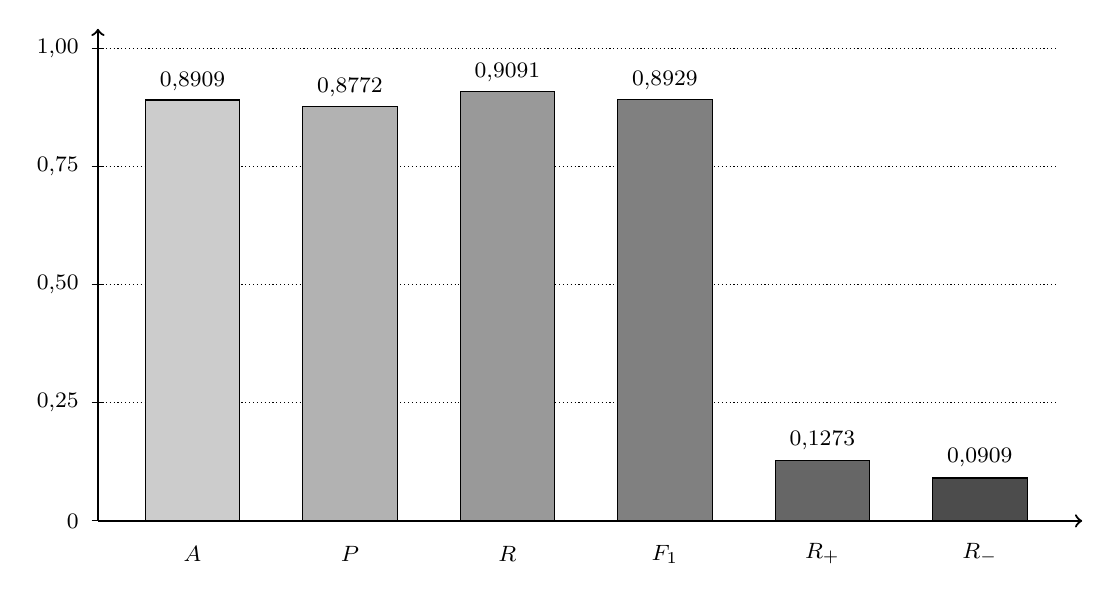
\begin{tikzpicture}[x=1cm,y=1cm]
  \draw[->,thick] (0,0) -- (0,6.25);
  \draw[->,thick] (0,0) -- (12.5,0);
  \foreach \y/\v in {0/0,1.5/0{,}25,3/0{,}50,4.5/0{,}75,6/1{,}00}{
    \draw (-0.08,\y) -- (0.08,\y);
    \node[anchor=east,font=\footnotesize] at (-0.12,\y) {\v};
    \draw[densely dotted] (0.1,\y) -- (12.2,\y);
  }
  \filldraw[fill=black!20,draw=black] (0.6,0) rectangle (1.8,5.3454);
  \filldraw[fill=black!30,draw=black] (2.6,0) rectangle (3.8,5.2632);
  \filldraw[fill=black!40,draw=black] (4.6,0) rectangle (5.8,5.4546);
  \filldraw[fill=black!50,draw=black] (6.6,0) rectangle (7.8,5.3574);
  \filldraw[fill=black!60,draw=black] (8.6,0) rectangle (9.8,0.7638);
  \filldraw[fill=black!70,draw=black] (10.6,0) rectangle (11.8,0.5454);

  \node[font=\footnotesize] at (1.2,5.58) {0,8909};
  \node[font=\footnotesize] at (3.2,5.50) {0,8772};
  \node[font=\footnotesize] at (5.2,5.69) {0,9091};
  \node[font=\footnotesize] at (7.2,5.59) {0,8929};
  \node[font=\footnotesize] at (9.2,1.02) {0,1273};
  \node[font=\footnotesize] at (11.2,0.80) {0,0909};

  \node[font=\footnotesize] at (1.2,-0.42) {$A$};
  \node[font=\footnotesize] at (3.2,-0.42) {$P$};
  \node[font=\footnotesize] at (5.2,-0.42) {$R$};
  \node[font=\footnotesize] at (7.2,-0.42) {$F_1$};
  \node[font=\footnotesize] at (9.2,-0.42) {$R_+$};
  \node[font=\footnotesize] at (11.2,-0.42) {$R_-$};
\end{tikzpicture}
\caption{Показники, арифметично одержані з агрегованої матриці помилок}
\label{fig:metric_comparison}
\end{figure}


Компонентне зіставлення попередньої експериментальної серії наведено в табл.~\ref{tab:ch4_component_results}. Перші чотири рядки характеризують окремі канали й спільну конфігурацію. Наступні три рядки відображають втручання в зафіксоване правило без повторного навчання. Їх не можна тлумачити як незалежне оцінювання нових скорочених моделей.

\begin{table}[htbp]
\caption{Агреговані результати окремих каналів і компонентного вилучення}
\label{tab:ch4_component_results}
\centering
\scriptsize
\resizebox{\textwidth}{!}{%
\begin{tabular}{lrrrrrr}
\toprule
Конфігурація & Правильність & Точність & Повнота & $F_1$ & Хибнопозитивні & Хибнонегативні \\
\midrule
Структурний канал & 0,6364 & 0,6027 & 0,8000 & 0,6875 & 0,5273 & 0,2000 \\
Канал спектральних і зорових ознак & 0,7273 & 1,0000 & 0,4545 & 0,6250 & 0,0000 & 0,5455 \\
Скорочена оцінка за правилами & 0,5000 & н/в* & 0,0000 & н/в* & 0,0000 & 1,0000 \\
Спільна конфігурація & 0,8909 & 0,8772 & 0,9091 & 0,8929 & 0,1273 & 0,0909 \\
\midrule
Без структурних ознак & 0,7545 & 1,0000 & 0,5091 & 0,6747 & 0,0000 & 0,4909 \\
Без спектральних і зорових ознак & 0,7364 & 0,8611 & 0,5636 & 0,6813 & 0,0909 & 0,4364 \\
Без скороченого вектора ознак, сформованих за правилами & 0,8909 & 0,8772 & 0,9091 & 0,8929 & 0,1273 & 0,0909 \\
\bottomrule
\end{tabular}}

\vspace{2pt}
\parbox{0.96\textwidth}{\footnotesize * Скорочена оцінка за правилами не сформувала жодного позитивного рішення, тому точність позитивного рішення й $F_1$ не визначені (ділення $0/0$); повнота при цьому дорівнює нулю коректно. Площу під характеристичною кривою не подано, бо для ретроспективної серії немає неперервних пооб’єктних оцінок.}
\end{table}

Після вилучення структурних ознак повнота зменшилася на $40{,}00$ відсоткового пункту, а після вилучення спектральних і зорових ознак --- на $34{,}55$ відсоткового пункту. Отже, зафіксоване правило було чутливим до обох статичних входів. Однак нульова заміна, відсутність повторного навчання та використання того самого набору для налаштування й оцінювання не дають змоги встановити причинний внесок кожної групи або статистичну значущість різниці.

Вилучення скороченого вектора ознак, сформованих за правилами, не змінило жодного агрегованого показника. Цей результат стосується лише доступної оцінки за правилами попередньої експериментальної серії. Він не підтверджує й не спростовує повний метод поведінкового узгодження ознак різного походження, оскільки причинно пов’язаних журналів $X_b$, повного представлення $Z_b$ та навченого механізму перехресного зіставлення не було.

Часові підсумки попередньої експериментальної серії наведено в табл.~\ref{tab:ch4_timing_results}. Середній сумарний час чотирьох операцій дорівнює $418{,}09$~мс. На операцію опрацювання спектральних і зорових ознак припадає $98{,}49$~\% цього часу; вона визначає часові витрати виміряної частини.

\begin{table}[htbp]
\caption{Агреговане зведення часу чотирьох операцій попередньої експериментальної серії}
\label{tab:ch4_timing_results}
\centering
\small
\resizebox{\textwidth}{!}{%
\begin{tabular}{lrrrr}
\toprule
Операція & Середнє, мс & Медіана, мс & 95-й процентиль, мс & Частка, \% \\
\midrule
Структурний аналіз & 5,82 & 4,71 & 15,68 & 1,39 \\
Аналіз спектральних і зорових ознак & 411,77 & 293,48 & 1511,46 & 98,49 \\
Скорочена оцінка за правилами & 0,36 & 0,31 & 0,53 & 0,09 \\
Інтеграція ознак & 0,14 & 0,13 & 0,19 & 0,03 \\
\midrule
Виміряна частина оброблення\textsuperscript{а} & 418,09 & 298,58 & 1530,80 & 100,00 \\
\bottomrule
\end{tabular}}

\vspace{2pt}
\parbox{0.96\textwidth}{\footnotesize \textsuperscript{а} Медіану та 95-й процентиль рядка «Виміряна частина оброблення» узято зі збереженого зведення попередньої експериментальної серії, де їх обчислено за розподілом пооб’єктних сум. Вони не дорівнюють сумі відповідних квантилів окремих операцій, оскільки квантилі не адитивні; середні значення, навпаки, додаються точно: $5{,}82+411{,}77+0{,}36+0{,}14=418{,}09$.}
\end{table}

Зі середнього $418{,}09$~мс арифметично випливає $2{,}39$ послідовно опрацьованого об’єкта за секунду. Це значення не є пропускною здатністю розгорнутої вебсистеми, оскільки не враховує приймання, чергу, прийняття рішення, реєстрацію, конкурентний доступ і передавання даних. Розподіл виміряного часу показано на рис.~\ref{fig:timing_breakdown}.

\begin{figure}[htbp]
\centering
\begin{tikzpicture}[x=0.13cm,y=1cm]
  \draw[fill=black!20,draw=black] (0,0) rectangle (1.39,1);
  \draw[fill=black!65,draw=black] (1.39,0) rectangle (99.88,1);
  \draw[fill=black!40,draw=black] (99.88,0) rectangle (99.97,1);
  \draw[fill=white,draw=black] (99.97,0) rectangle (100,1);
  \draw[thick] (0,0) rectangle (100,1);
  \node[white,font=\footnotesize] at (50.635,0.5)
    {аналіз спектральних і піксельних ознак: 98,49\%};
  \draw[->] (0.695,1.05) -- (8,2.1);
  \node[anchor=west,font=\footnotesize] at (8,2.1)
    {структурний аналіз: 1,39\%};
  \draw[->] (99.925,-0.05) -- (75,-1.05);
  \node[anchor=east,font=\footnotesize,align=right] at (75,-1.05)
    {оцінка ознак подій і поведінки за правилами: 0,09\%;\\інтеграція ознак: 0,03\%};
  \node[anchor=west,font=\footnotesize] at (0,-0.55) {0\%};
  \node[anchor=east,font=\footnotesize] at (100,-0.55) {100\%};
  \node[font=\footnotesize] at (50,-1.65)
    {прийняття рішення та реєстрацію результатів не враховано};
\end{tikzpicture}
\caption{Розподіл середнього часу між виміряними операціями}
\label{fig:timing_breakdown}
\end{figure}


Окреме категоріальне зведення попереднього опису дає зважене середнє $424{,}72$~мс, яке не збігається з операційним значенням $418{,}09$~мс. Без первинного часового журналу неможливо встановити, чи спричинена різниця складом груп, порядком усереднення або різними запусками. Тому категоріальне середнє не використано для висновку, а часові результати ретроспективного й внутрішнього циклів не зіставляються як показник прискорення.

У першій зовнішній серії середній виміряний час формування структурних, спектральних і зорових ознак для стандартизованого 12-кадрового фрагмента становив $830{,}268$~мс, а для повного первинного MP4 --- $18\,187{,}221$~мс. Ці значення не зіставляються як оцінка прискорення або уповільнення, оскільки фрагменти й повні записи відрізнялися тривалістю та просторовою роздільністю. Вони показують, що збільшення кількості декодованих кадрів безпосередньо збільшує вартість аналізу спектральних і зорових ознак і має враховуватися під час вибору між синхронним опрацюванням та попередньою ізоляцією відеоматеріалу.

Загальна тривалість службових запусків не використовується як показник швидкодії. Вона залежала від повторного використання підготовлених об’єктів, кількості робочих потоків, перевірки контрольних сум і формування звітів. Для порівняння конфігурацій застосовано лише однопотокове ресурсне вимірювання на однаковій підмножині, наведене в табл.~\ref{tab:ch4_rating_results}.

Предметне тлумачення результатів визначається межами протоколу. За підсумковим описом внутрішній цикл передбачав груповий поділ без змішування похідних спільного походження, однак повного реєстру для незалежної перевірки поділу й пооб’єктних оцінок не збережено; базові сцени були синтетичними, а види змін --- наперед відомими. Чотири зовнішні набори разом охопили $38$ реальних відеозаписів із $12$ пристроїв, проте тисячі похідних залишаються залежними від малої кількості джерел. Ретроспективний цикл характеризує попередню конфігурацію, але не має незалежного поділу й повного первинного журналу. Основні межі систематизовано в табл.~\ref{tab:ch4_validity_limits}.

{\small
\begin{longtable}{@{}p{0.23\textwidth}p{0.34\textwidth}p{0.34\textwidth}@{}}
\caption{Межі тлумачення експериментальних результатів}\label{tab:ch4_validity_limits}\\
\toprule
Аспект & Установлена межа & Наслідок для висновку \\
\midrule
\endfirsthead
\multicolumn{3}{l}{Продовження таблиці \thetable}\\
\toprule
Аспект & Установлена межа & Наслідок для висновку \\
\midrule
\endhead
\bottomrule
\endfoot
Походження даних & Внутрішній набір за підсумковим описом є синтетичним і не має повного пооб’єктного реєстру; зовнішні набори містять $38$ реальних відеозаписів із $12$ пристроїв; ретроспективний набір також не має повного реєстру & Оцінено перенесення на нові записи, але не встановлено універсальності для довільних пристроїв, сцен і способів кодування; внутрішній груповий поділ не перевірено на рівні сирих записів \\
Залежність спостережень & $56$, $32$, $10\,000$ і $2\,000$ похідних утворено відповідно з $8$, $4$, $4$ і $8$ груп «пристрій--сцена», тобто разом із $24$ зовнішніх груп походження; дві останні серії додатково поділено на $500$ і $100$ базових фрагментів. Загалом зовнішні набори охоплюють $38$ реальних відеозаписів із $12$ пристроїв & Кількість похідних не можна прирівнювати до кількості незалежних джерел; повторне вибирання виконано за групами й вихідними записами, а умовні інтервали характеризують саме наявні записи \\
Предмет позитивної мітки & Мітка позначає контрольовану структурну або статистичну зміну & Не підтверджено виявлення або виконання аномального програмного коду \\
Охоплення форматів & PNG, JPEG, WebP, MP4 і WebM оцінено в багатоформатній та заздалегідь відокремленій зовнішній серіях; для JPEG, WebP і WebM виконано перенесення без повторного навчання & Підтверджено працездатність у заданих умовах, але не всі кодеки, профілі та реалізації форматів \\
Структурні контрольні приклади & У розвідувальному аналізі $1\,500$ допустимо змінених контрольних об’єктів усі об’єкти пройшли розбір і декодування; $1\,000$ контейнерних пар були піксельно тотожними. Для приватних розширень або відступів частка хибнопозитивних рішень становила $1{,}0000$ у кожному з п’яти форматів & Структурна гілка виявляє заданий формальний індикатор, але не відокремлює його від усієї допустимої контейнерної варіативності; позитивне рішення потребує перевірки відповідності формату й правилам безпеки, а також експертної оцінки \\
Збереження спектрального сліду & У ретроспективному парному аналізі $2\,500$ форматних пар кожна спектральна умова мала ненульову декодовану відмінність; середній PSNR становив від $38{,}6417$ до $41{,}4147$~дБ, а $5\,000$ контейнерних контрольних пар були піксельно тотожними. Передкодувальні просторово-часові маски не збережено & Повне зникнення сліду не пояснює низького результату ізольованої гілки; підтверджено невідповідність агрегованих ознак малому розсіяному залишку, але не виміряно збереження первинної локалізації \\
Охоплення сценаріїв & Модель узгодження не виявила жодної з $500$ суто спектральних змін заздалегідь відокремленої зовнішньої серії & Висока специфічність і збалансований показник не доводять придатності до всіх видів прихованого впливу \\
Дані про події та поведінку & У $4\,832$ фізично окремих похідних відеооб’єктах, які не є незалежними джерелами, доступна технічна ознака не спрацювала; журнали $X_b$ і повне $Z_b$ не сформовано & Перевірено узгодження статичних оцінок, але не повний метод поведінкового узгодження і не повне представлення $Z$ \\
Відтворення параметрів і результатів & Для зовнішніх серій та моделі узгодження збережено код, протоколи, параметри, реєстри й прогнози; відновлений набір параметрів першого методу чисельно відтворює зовнішні архівні оцінки, але не є побайтовою копією відсутнього первинного артефакту. Для внутрішніх $400$ об’єктів немає повного реєстру, ознак, оцінок, повторних вибірок і сирих часових записів. Первинного модуля виділення спектральних ознак і сталого публічного ідентифікатора пакета також немає & Для зовнішніх серій відтворено застосування моделей, повторне навчання моделі узгодження та числові підсумки; для внутрішньої серії перевіряється лише арифметика агрегованих матриць і похідних показників. Не підтверджено внутрішні AUC та інтервали, тотожне наскрізне історичне виділення ознак і довготривалу доступність пакета \\
Ресурсне оцінювання & Час і пам’ять конфігурацій виміряно в п’яти однопотокових запусках; окремий локальний аудит охопив один чотирипроцесний запуск десяти об’єктів & Значення придатні для внутрішнього порівняння та перевірки локальної завершеності, але не визначають тривалої пропускної здатності розгорнутої вебсистеми \\
Технологічні стани й відмови & У $45$ сценарних спостереженнях перевірено штатний цикл, $m_b=0$, помилку декодування, відмову атомарної реєстрації, повтор, відновлення та чотирипроцесний запуск; створено $35$ цілісних записів $S_5$ & Підтверджено локальні переходи й безпечне завершення, але не реконструкцію, виконання зовнішніх приписів, розподілену чергу, мережеву взаємодію або промислову готовність \\
Інтегральний рейтинг & Формулу $K_I$ сформовано після первинного перегляду якості, її складники залежні, а ресурсну частину оцінено на підмножині даних розроблення & Рейтинг є розвідувальним; його потрібно наперед зафіксувати й підтвердити на нових джерелах і незалежному ресурсному запуску \\
\end{longtable}
}

Інтегральний рейтинг $K_I$ не утворюється механічним об’єднанням результатів шести серій. Його обчислено лише для конфігурацій, які пройшли єдине багатоформатне й ресурсне оцінювання. Ретроспективне значення $0{,}8909$, внутрішнє значення $0{,}9750$ і результати заздалегідь відокремленої зовнішньої серії мають інші одиниці аналізу та не входять до одного бала. Завдяки цьому $K_I$ характеризує конкретний сценарій вибору, а не всю інформаційну технологію.

Послідовність серій змінила початковий висновок. У синтетичному наборі спільна проєкція $Z_c$ усунула більшість помилок ізольованої конфігурації спектральних і зорових ознак. Перша зовнішня серія не відтворила її переваги над структурною конфігурацією. Багатоформатна серія, зі свого боку, виявила межу вже структурної конфігурації на WebM і показала, що спільна проєкція має рівномірніший форматний профіль. Модель узгодження усунула хибнопозитивні рішення на нових пристроях, але знизила повноту й не виявила суто спектральних змін. Отже, жодна конфігурація не є безумовно найкращою: структурна мінімізує ресурсні витрати, спільна зберігає більшу повноту, а модель узгодження надає перевагу специфічності.

Відсутність спрацювання ознаки подій і поведінки у $4\,832$ фізично окремих похідних відеооб’єктах, які не є незалежними джерелами, пояснює, чому результати моделі узгодження визначалися статичними оцінками. Це не свідчить про нульову цінність причинно пов’язаних подій, яких у дослідженні не було. Для перевірки повного другого методу потрібні парні журнали штатного й зміненого оброблення того самого об’єкта, причинне пов’язування подій із фазами, визначення параметрів кодувальника лише за навчальною частиною та одноразове оцінювання на нових групах.

Отже, експерименти підтвердили чутливість структурного аналізу до заданих контейнерних втручань, але контрольний аналіз допустимої варіативності виявив недостатню специфічність цього індикатора. Установлено форматну межу перенесення, кількісно описано компроміс між специфічністю, повнотою та ресурсними витратами, оцінено скорочену модель узгодження статичних оцінок у заздалегідь відокремленій зовнішній серії та перевірено локальні переходи $S_1$--$S_5$ із безпечним завершенням за двох класів технічних відмов. Межі тлумачення наведено в табл.~\ref{tab:ch4_validity_limits}: не підтверджено відокремлення загрозливих структур від усіх допустимих варіантів контейнера, повний контур узгодження статичних ознак з ознаками подій і поведінки, виявлення виконуваного аномального коду чи промислову готовність. Практичне застосування на цьому етапі має передбачати перевірку відповідності формату й правилам безпеки, а також експертну оцінку позитивного рішення, а не безумовне автоматичне блокування.

\section*{Висновки до розділу 4}
\phantomsection
\addcontentsline{toc}{section}{Висновки до розділу 4}

\begin{enumerate}[label=\arabic*.]
\item Експериментальне дослідження охопило шість серій, окреме ресурсне вимірювання та локальний аудит технологічних станів. За підсумковим описом внутрішня серія містила $200$ первинних груп і $400$ PNG- та MP4-об’єктів із поділом $60:20:20$; повний пооб’єктний реєстр цієї серії не збережено. Чотири зовнішні набори містили $38$ неповторюваних реальних відеозаписів із $12$ пристроїв; багатоформатна серія охопила $10\,000$ похідних, а заздалегідь відокремлена зовнішня серія --- $2\,000$. Кількість похідних не прирівнювалася до кількості незалежних джерел.

\item За збереженим підсумком внутрішньої перевірної частини з $80$ об’єктів спільна числова проєкція $Z_c$ дала $40$ правильно визначених контрольних, жодного хибнопозитивного, два хибнонегативні та $38$ правильно визначених змінених об’єктів. Із матриці повторно обчислюються частка правильних рішень $0{,}9750$, повнота $0{,}9500$ і $F_1=0{,}9744$; повідомлену площу $0{,}9869$ без неперервних оцінок незалежно не перевірено. Числова перевага над конфігурацією спектральних і зорових ознак була виразною, тоді як парна відмінність від структурної конфігурації не досягла рівня $0{,}05$ ($p=0{,}0625$). Отже, агреговані підсумки підтримують корисність структурних ознак як доповнення до $Z_v$, але не доводять загальної переваги $Z_c$ над $Z_s$.

\item Перша зовнішня серія на $56$ похідних MP4 не відтворила внутрішньої переваги спільної проєкції над структурною конфігурацією. Для $Z_s$ збалансована частка правильних рішень становила $0{,}8333$, для $Z_c$ --- $0{,}7857$, а для $Z_v$ --- $0{,}5000$. На цьому етапі саме структурне свідчення збереглося після переходу до реальних MP4, тоді як перенесення роздільної здатності реалізованих спектральних і зорових ознак не підтверджено.

\item Багатоформатна серія показала, що структурна конфігурація, конфігурація спектральних і зорових ознак та спільна конфігурація мають збалансовані частки правильних рішень $0{,}7636$, $0{,}5001$ і $0{,}7916$. Структурна конфігурація дала $0{,}5000$ на WebM, тоді як спільна проєкція мала форматні значення від $0{,}7387$ до $0{,}8173$. Отже, висновок першої MP4-серії не переноситься безумовно на всі формати. Класичні статистичні показники окремо залишилися поблизу $0{,}5$ і не забезпечили виконання форматної умови після об’єднання зі структурним рішенням.

\item У заздалегідь відокремленій зовнішній серії точкове значення збалансованої частки правильних рішень моделі узгодження змінилося від $0{,}7827$ до $0{,}8307$. Модель усунула $76$ хибнопозитивних рішень, але додала $84$ пропуски, зменшила загальну частку правильних рішень від $0{,}7500$ до $0{,}7460$ та не виявила жодної з $500$ суто спектральних змін. Критерій Мак-Немара дав $p=0{,}5801$. Отже, відтворено профіль із пріоритетом специфічності, а не безумовну перевагу за всіма показниками.

\item Недеструктивне повторне виділення ознак із тих самих $56$ і $2\,000$ файлів MP4 поточною еталонною реалізацією повністю зберегло структурні рішення: збалансована частка правильних рішень $Z_s$ залишилася $0{,}8333$. Для $Z_v$ вона залишилася поблизу випадкового рівня, а для $Z_c$ зменшилася відповідно від $0{,}7857$ до $0{,}6905$ і від $0{,}7987$ до $0{,}6520$ через зсув співвідношення специфічності та повноти. Отже, відтворено структурну частину, але не числову тотожність модуля виділення спектральних ознак; архівні результати потрібно тлумачити за канонічними таблицями ознак.

\item Розвідувальний аналіз $1\,500$ допустимо змінених контрольних об’єктів показав, що для приватних розширень або відступів частка хибнопозитивних структурних рішень дорівнювала $1{,}0000$ у кожному з п’яти форматів, хоча всі об’єкти пройшли розбір і декодування, а декодований вміст залишився тотожним початковому. Для повторного кодування або компонування частка становила $0{,}4040$ загалом і $1{,}0000$ для JPEG та WebM. Отже, $Z_s$ є індикатором заданої формальної ознаки контейнера, але не самодостатнім доказом прихованого впливу; потрібні репрезентативні допустимі структури під час нового навчання та окрема перевірна вибірка.

\item Розвідувальний парний аналіз $2\,500$ представлень у форматах PNG, JPEG, WebP, MP4 і WebM установив ненульову декодовану відмінність для кожної спектральної умови. Середній за відеоджерелами PSNR становив від $38{,}6417$ до $41{,}4147$~дБ, тоді як усі $5\,000$ контейнерних контрольних пар були піксельно тотожними. Отже, низький результат $Z_v$ не пояснюється повним зникненням сліду; реалізовані агреговані ознаки не забезпечили стійкого розрізнення малого розсіяного залишку. Через відсутність масок, збережених до кодування, просторове збереження первинної зміни не встановлено.

\item Ресурсне вимірювання в п’яти окремих запусках процесу дало 95-ті процентилі $2{,}136$, $760{,}662$, $853{,}971$ і $1078{,}904$~мс та значення пам’яті $78{,}77$, $96{,}79$, $101{,}53$ і $110{,}05$~МіБ відповідно для структурної конфігурації, конфігурації спектральних і зорових ознак, спільної конфігурації та моделі узгодження. Розвідувальний $K_I$ становив $77{,}50$, $50{,}69$, $68{,}95$ і $69{,}46$. Структурна конфігурація посіла перше місце завдяки швидкодії, але не виконала форматної умови; тому інтегральний бал тлумачиться лише разом із первинними складниками.

\item Ретроспективна перевірка $110$ об’єктів установила арифметичну узгодженість матриці $48$, $7$, $5$, $50$ та похідних від неї показників: правильності $0{,}8909$, точності позитивного рішення $0{,}8772$, повноти $0{,}9091$ і $F_1=0{,}8929$. Площу під характеристичною кривою не подано через відсутність пооб’єктних оцінок, а компонентне вилучення характеризує лише чутливість зафіксованого правила. Середній час $418{,}09$~мс стосується чотирьох операцій попередньої конфігурації; внутрішні $53{,}89$~мс для PNG і $198{,}76$~мс для MP4 є збереженими підсумковими значеннями без сирих часових записів, а зовнішні $830{,}268$~мс для 12-кадрового фрагмента охоплюють лише формування статичних ознак.

\item За наперед зафіксованим протоколом одержано $45$ спостережень локального технологічного циклу: $35$ циклів завершилися цілісним $S_5$, а п’ять помилок декодування і п’ять контрольовано внесених відмов реєстрації безпечно завершилися без $S_5$ та без зовнішньої дії. Штатні цикли зберегли порядок $S_1$--$S_5$, незмінність SHA-256 входу, $m_b=0$ за відсутності $J_b$ та розділення $S_A$ і $D_A$; повтор і відновлення отримали нові ідентифікатори. Один чотирипроцесний запуск десяти об’єктів завершився без пошкоджених записів із пропускною здатністю $22{,}827$ об’єкта за секунду та найбільшою сукупною пам’яттю $545{,}52$~МіБ. Результат підтверджує локальну реалізацію переходів і відмов, але не промислову масштабованість.

\item Повну конфігурацію методу поведінкового узгодження експериментально не перевірено: причинно пов’язані журнали $X_b$ і повне представлення $Z_b$ не сформовано, а доступна технічна ознака не спрацювала у $4\,832$ фізично окремих похідних відеооб’єктах, які не є незалежними джерелами. Позитивна мітка позначала контрольовану зміну, а не виконання аномального коду. Перенесення перевірено для п’яти форматів, але реконструкція, зовнішні дії у відповідь, розподілена черга, мережеве передавання та тривале промислове навантаження залишаються поза межами одержаного підтвердження.
\end{enumerate}
